\documentclass{article}
\usepackage[main,final,nonatbib]{neurips_2025}

\usepackage[utf8]{inputenc}
\usepackage[T1]{fontenc}
\usepackage{hyperref}
\usepackage{url}
\usepackage{booktabs}
\usepackage{graphicx}
\usepackage{amsmath}
\usepackage{microtype}
\usepackage{xcolor}
\usepackage{enumitem}
\usepackage{float}
\usepackage{adjustbox}

\title{DSAA2011 Covertype Project Report}

\author{%
  Covertype Project Team\\
  DSAA2011 Machine Learning Course Project\\
  \texttt{groupID\_covertype}\\
}

\begin{document}
\maketitle

\begin{abstract}
This report studies the UCI Covertype dataset with 581,012 forest observations, 54 cartographic features, and seven cover-type classes. The analysis covers preprocessing, t-SNE visualization, MiniBatchKMeans and Ward clustering, supervised classification, model validation, a Wilderness Area extension, feature importance, calibration, robustness, and computational optimization. Natural clusters reveal terrain and region structure but do not recover the seven ecological labels. A Random Forest classifier is the strongest predictive model on the stratified test set, achieving accuracy=0.902, macro-F1=0.845, and macro one-vs-rest AUC=0.991.
\end{abstract}

\section{Introduction}
The Covertype task predicts forest cover type from cartographic variables. The target is imbalanced: Lodgepole Pine and Spruce/Fir account for most observations, while Cottonwood/Willow is only 0.5\% of the data. We therefore report macro-averaged metrics in addition to accuracy. The main empirical result is that unsupervised structure is visible but does not directly match the supervised label definition, whereas nonlinear supervised ensembles perform well.

\begin{table}[H]
\centering
\caption{Class distribution in the Covertype dataset.}
\label{tab:target}
\small
\begin{adjustbox}{max width=\linewidth}
\begin{tabular}{llll}
\toprule
Cover\_Type & Cover\_Type\_Name & count & proportion \\
\midrule
1 & Spruce/Fir & 211,840 & 36.5\% \\
2 & Lodgepole Pine & 283,301 & 48.8\% \\
3 & Ponderosa Pine & 35,754 & 6.2\% \\
4 & Cottonwood/Willow & 2,747 & 0.5\% \\
5 & Aspen & 9,493 & 1.6\% \\
6 & Douglas-fir & 17,367 & 3.0\% \\
7 & Krummholz & 20,510 & 3.5\% \\
\bottomrule
\end{tabular}
\end{adjustbox}
\end{table}

\section{Data preprocessing}
The raw UCI file is numeric and has no header. We assign the official feature names, use 10 continuous terrain measurements, 4 wilderness-area indicators, 40 soil-type indicators, and the seven-class \texttt{Cover\_Type} target. There are no missing values. Continuous features are standardized for linear and distance-based methods; binary indicators are kept as indicator variables. The implemented data optimization uses \texttt{float32} for continuous variables and \texttt{uint8} for indicators and target, reducing the naive all-\texttt{int64} memory estimate from 243.8 MB to 47.1 MB.

\begin{figure}[H]
\centering
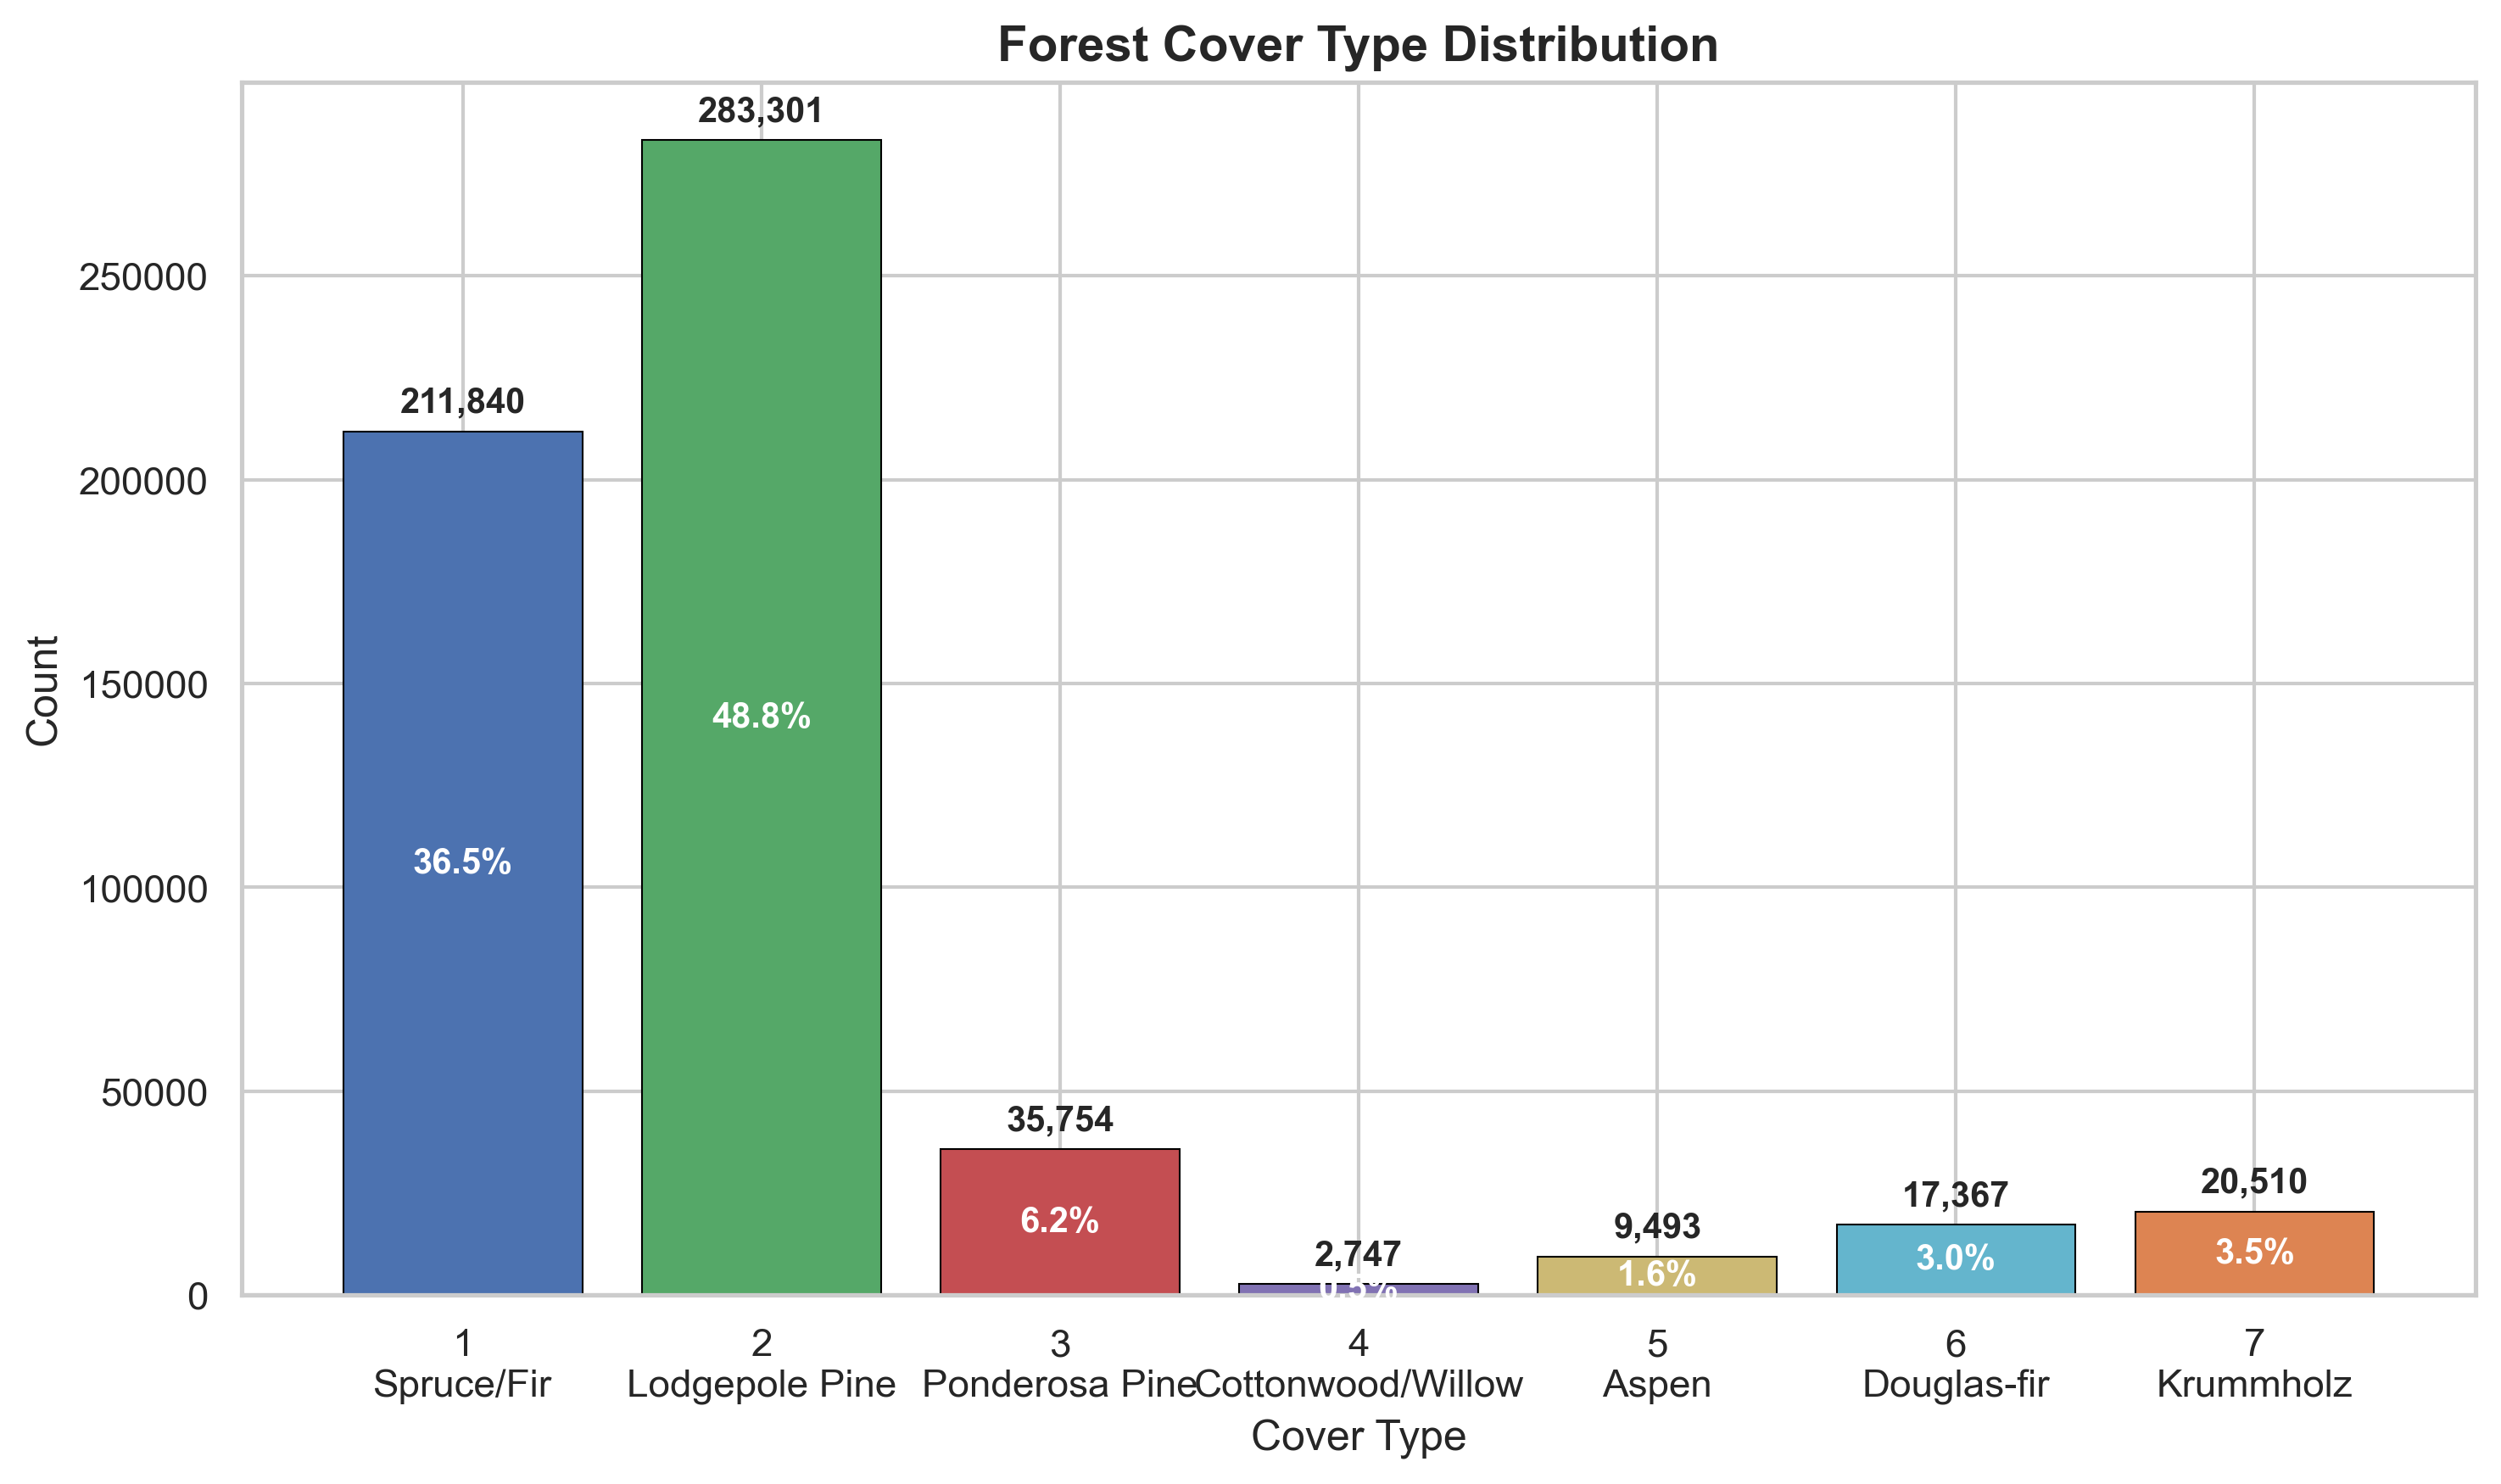
\includegraphics[width=0.78\linewidth]{figures/target_distribution.png}
\caption{Cover-type distribution. The two dominant classes make macro metrics necessary.}
\label{fig:target}
\end{figure}

\section{Visualization and clustering}
t-SNE is applied to a stratified 6,000-row sample after standardization and PCA compression to 30 dimensions. The embedding shows partial local separation for high-elevation classes, but Spruce/Fir and Lodgepole Pine overlap substantially. This motivates supervised classification rather than relying on natural clusters.

MiniBatchKMeans and Ward hierarchical clustering are evaluated with silhouette, Calinski-Harabasz, adjusted Rand index against \texttt{Cover\_Type}, and adjusted Rand index against \texttt{Wilderness\_Area}. MiniBatchKMeans is used as the scalable K-Means variant; Ward is restricted to a smaller structural sample because of its quadratic memory/time behavior. The near-zero ARI against \texttt{Cover\_Type} should not be read as a failure to find any structure. It shows that the strongest unsupervised partitions are not equivalent to the seven ecological labels; the clusters are better interpreted as coarse terrain or regional groupings.

\begin{figure}[H]
\centering
\begin{minipage}{0.48\linewidth}\centering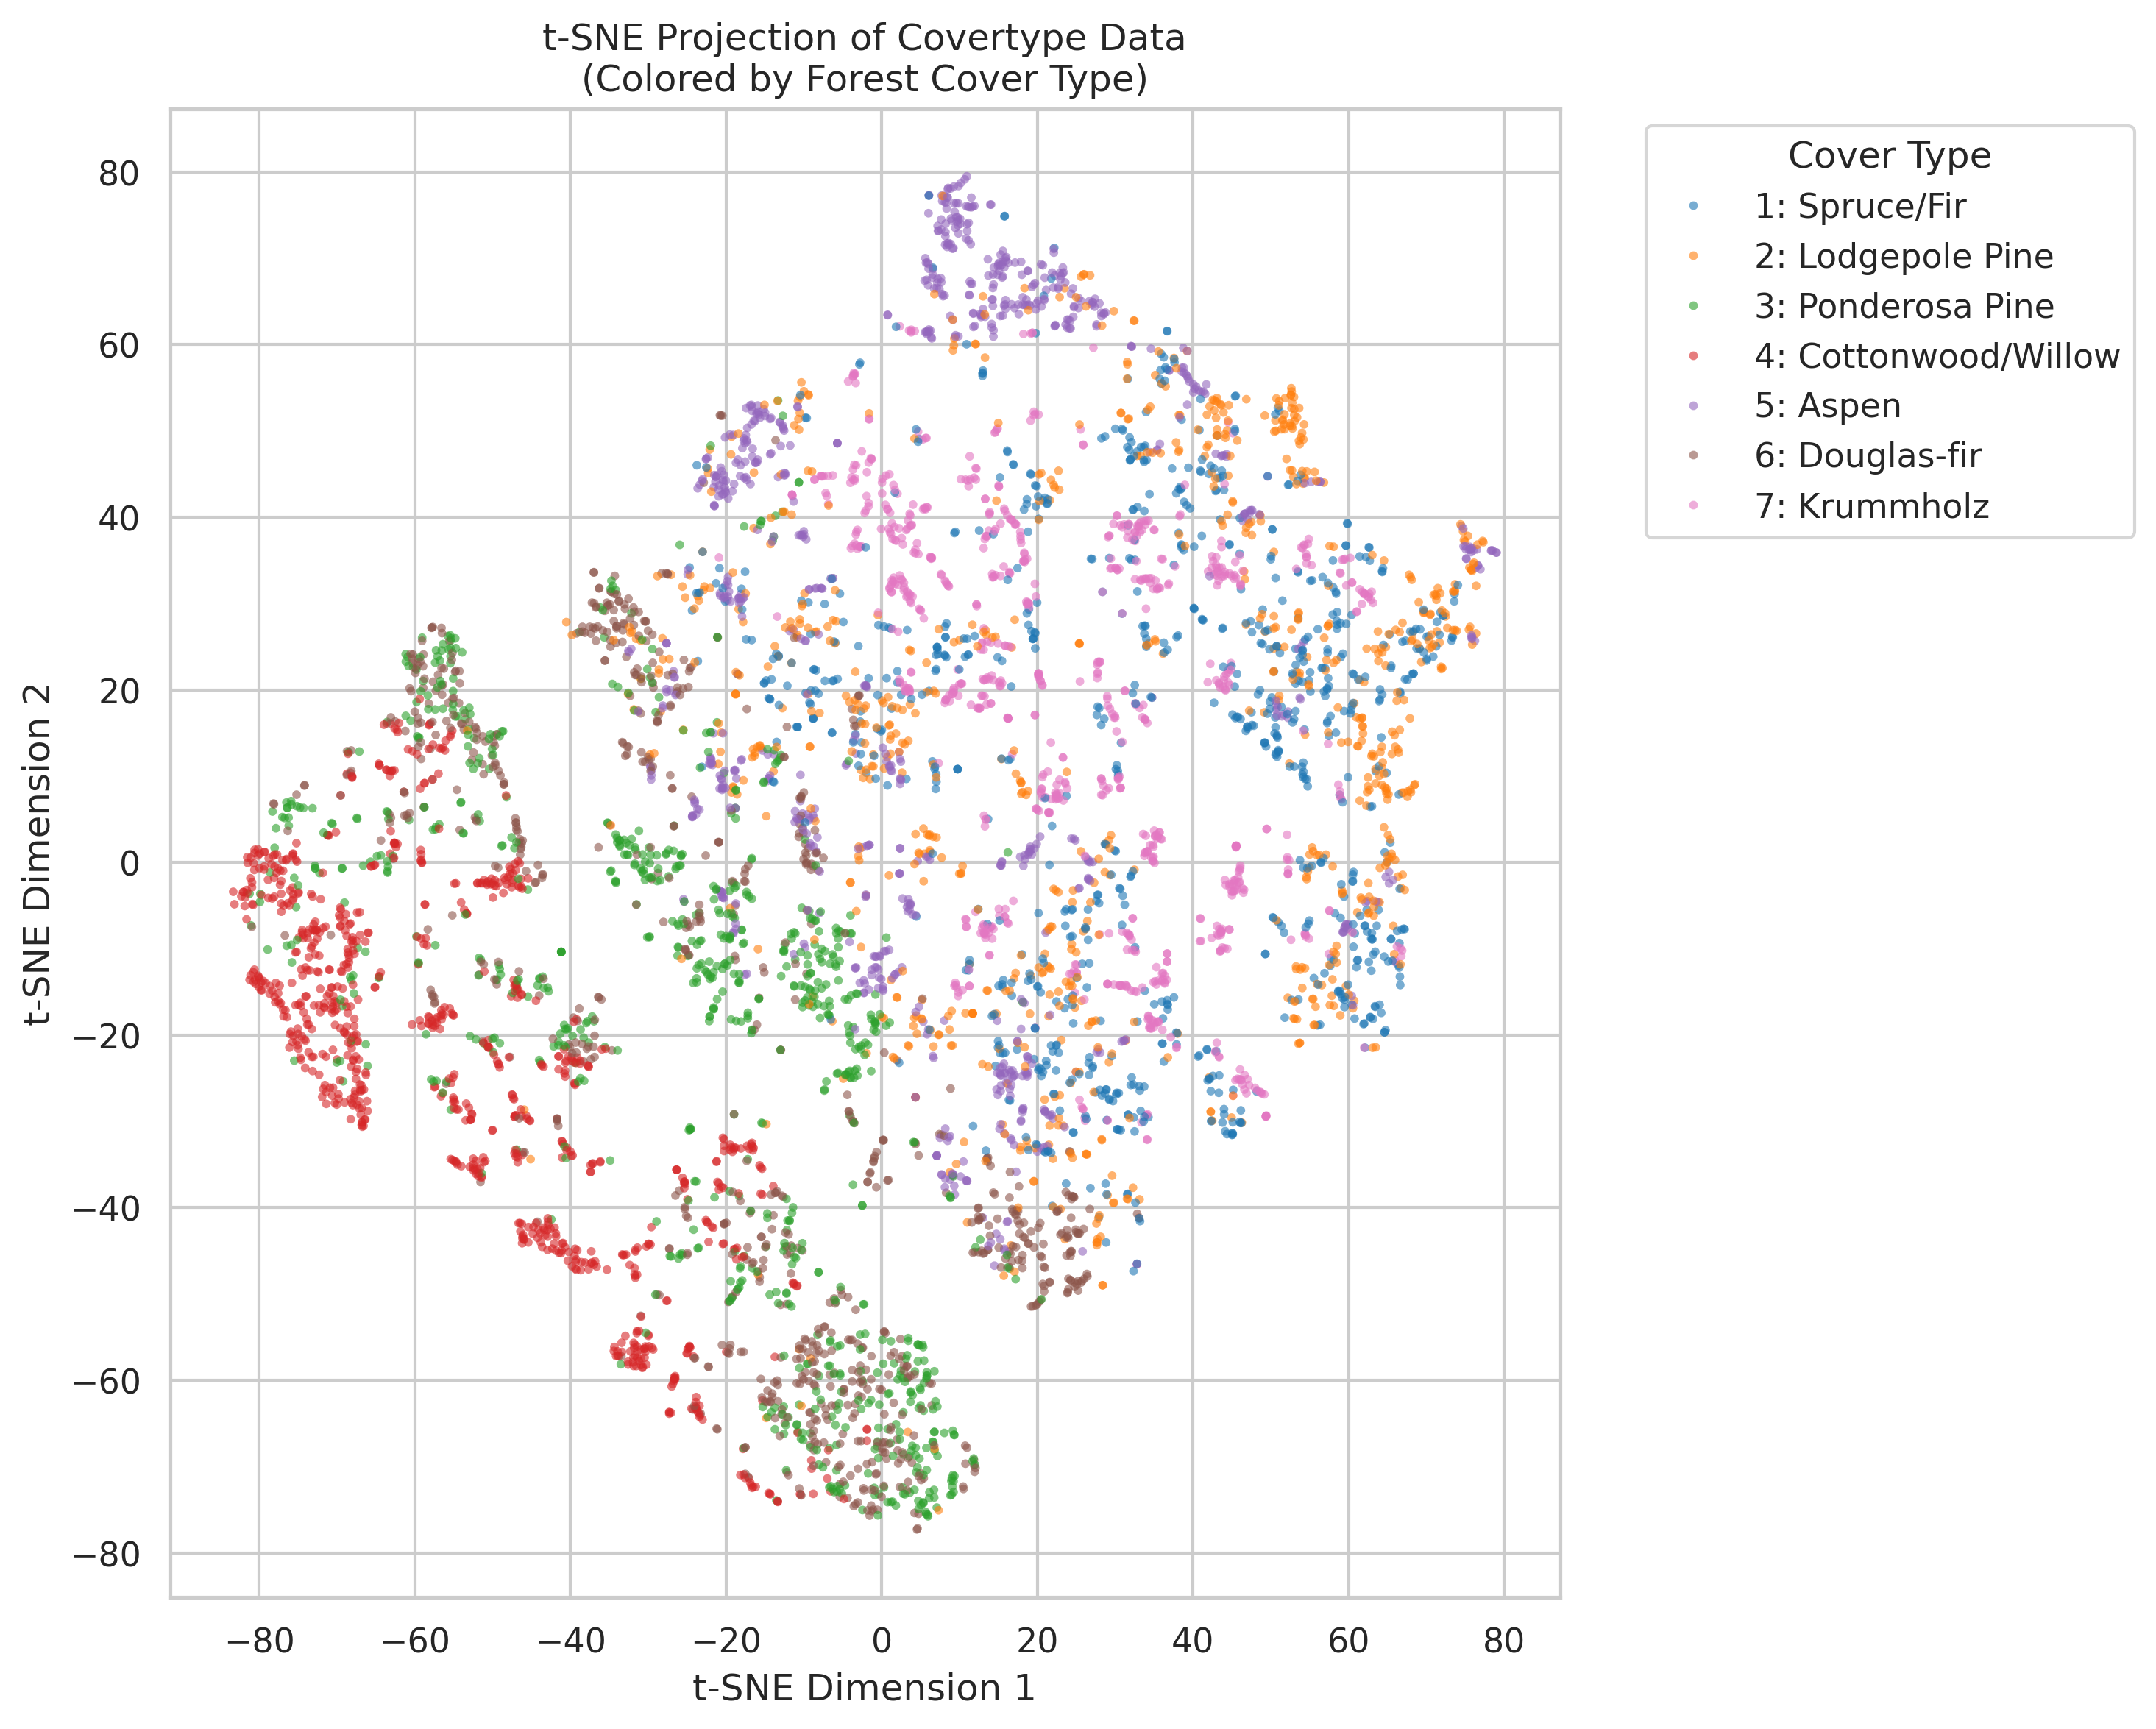
\includegraphics[width=\linewidth]{figures/tsne_target.png}\\[-0.5ex]\small t-SNE by target\end{minipage}\hfill%
\begin{minipage}{0.48\linewidth}\centering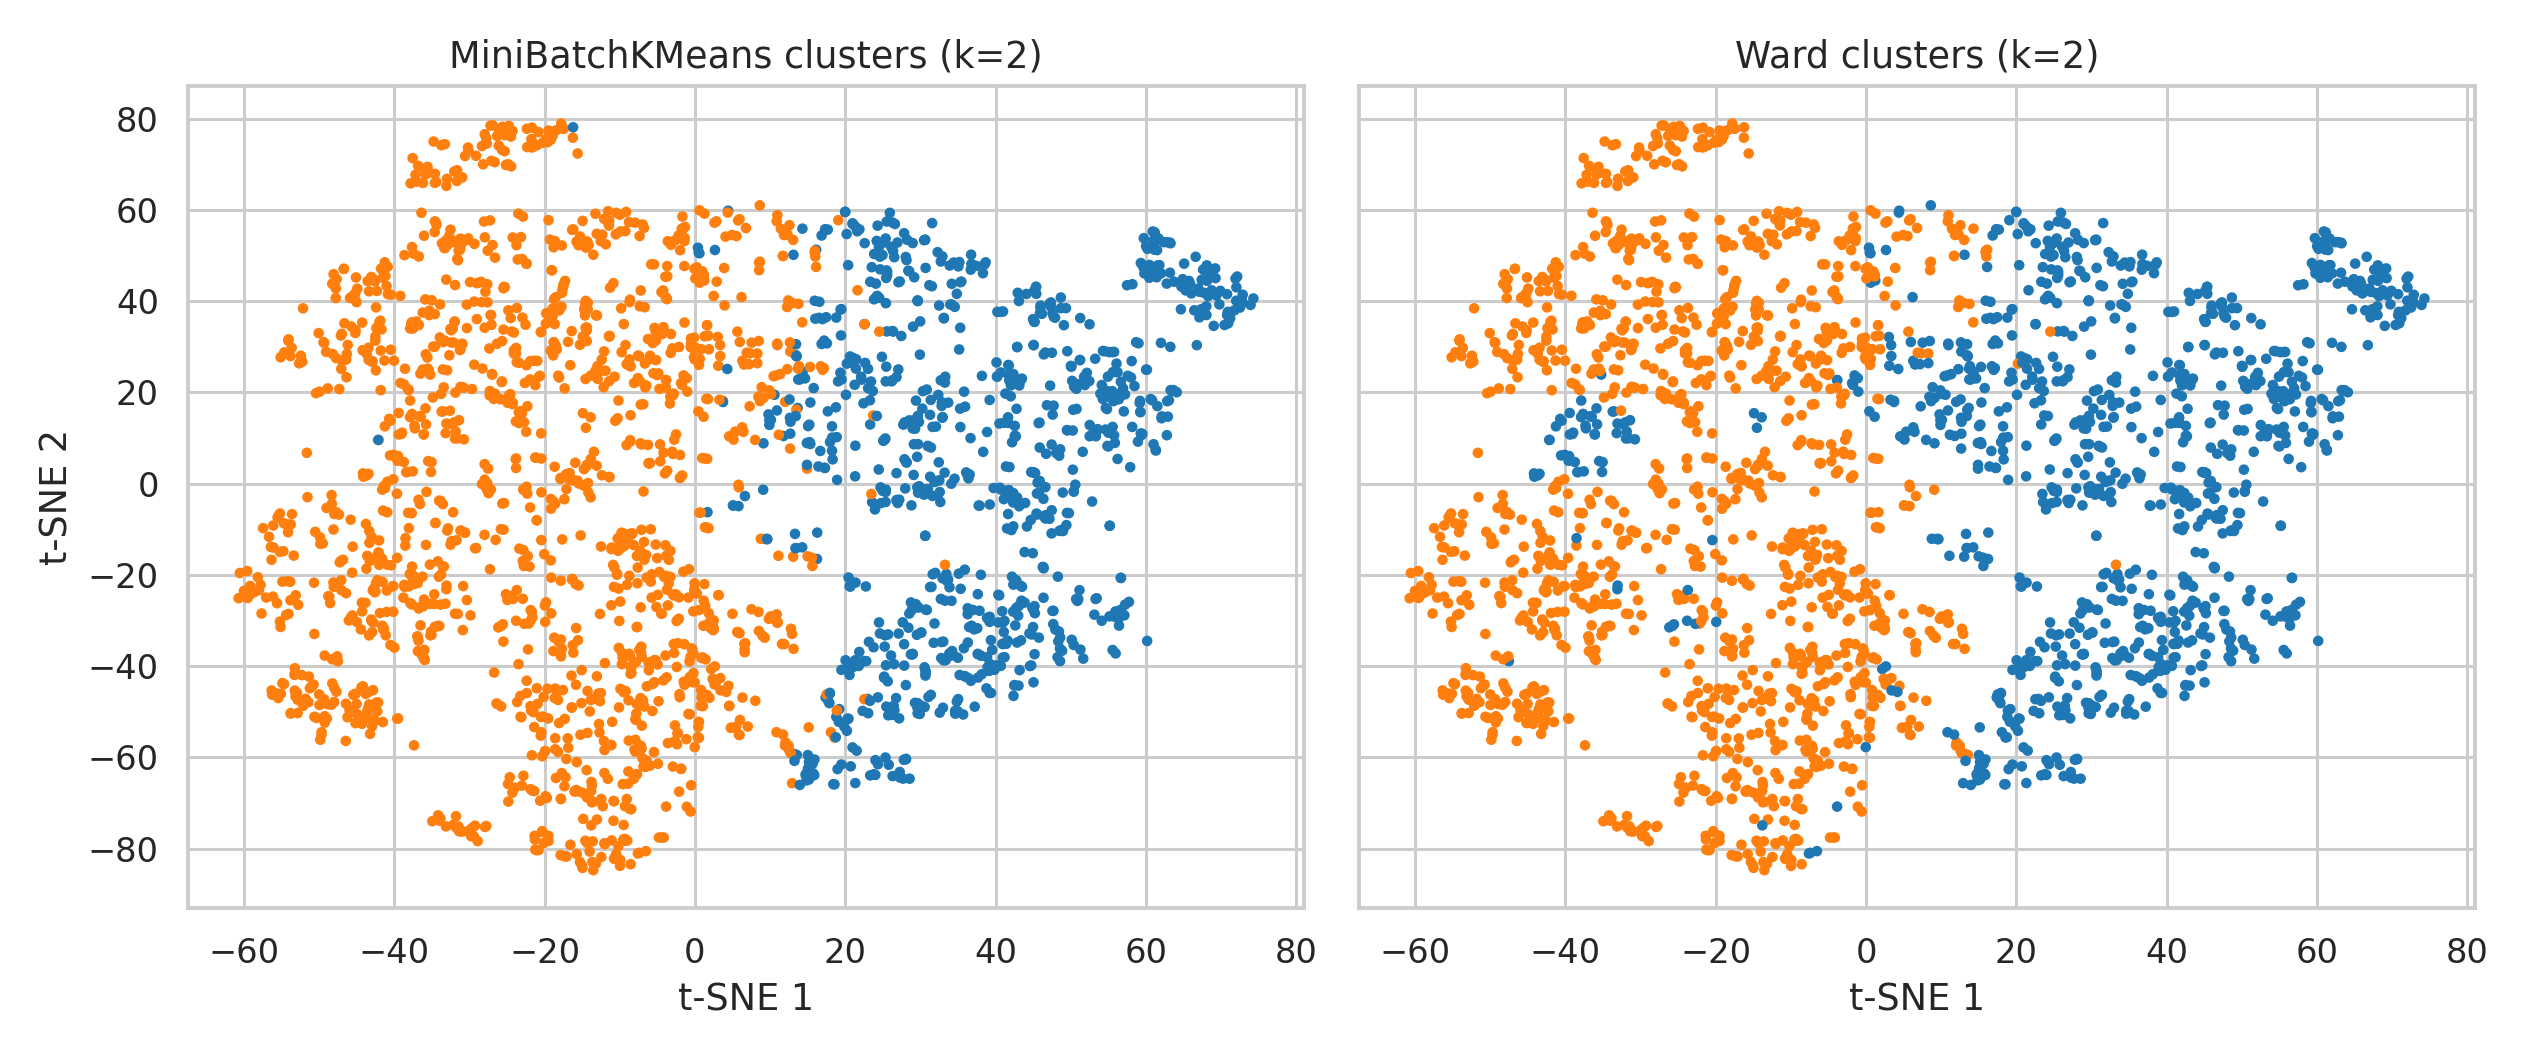
\includegraphics[width=\linewidth]{figures/clustering_tsne.png}\\[-0.5ex]\small Cluster assignments\end{minipage}
\caption{Low-dimensional visualization and clustering results.}
\label{fig:viz_cluster}
\end{figure}

\begin{table}[H]
\centering
\caption{Best clustering results under the selected internal metrics.}
\label{tab:cluster}
\small
\begin{adjustbox}{max width=\linewidth}
\begin{tabular}{llllll}
\toprule
algorithm & k & silhouette & CH & ARI target & ARI wild \\
\midrule
MiniBatchKMeans & 2 & 0.191 & 1340.066 & 0.003 & 0.039 \\
Agglomerative Ward & 2 & 0.153 & 406.143 & 0.004 & 0.013 \\
\bottomrule
\end{tabular}
\end{adjustbox}
\end{table}

\section{Wilderness Area extension}
The four one-hot wilderness indicators are converted into a compact \texttt{Wilderness\_Area} variable. This gives an additional explanatory view that is distinct from the seven-class prediction target. The areas differ strongly in size and cover-type composition: each wilderness area has a dominant cover type, but the normalized entropy shows that some areas contain more mixed ecological labels than others. This supports the revised clustering interpretation: low ARI versus \texttt{Cover\_Type} only says that natural clusters are not the target labels; it does not rule out meaningful structure associated with region, elevation, and terrain.

\begin{table}[H]
\centering
\caption{Cover-type composition summary by wilderness area.}
\label{tab:wilderness_summary}
\small
\begin{adjustbox}{max width=\linewidth}
\begin{tabular}{lllllll}
\toprule
area & name & n & share & dominant cover & dominant share & entropy \\
\midrule
1 & Rawah & 260,796 & 44.9\% & Lodgepole Pine & 56.1\% & 0.426 \\
2 & Neota & 29,884 & 5.1\% & Spruce/Fir & 62.2\% & 0.439 \\
3 & Comanche Peak & 253,364 & 43.6\% & Lodgepole Pine & 49.4\% & 0.628 \\
4 & Cache la Poudre & 36,968 & 6.4\% & Ponderosa Pine & 58.0\% & 0.547 \\
\bottomrule
\end{tabular}
\end{adjustbox}
\end{table}

The same held-out predictions from the best supervised model are then grouped by wilderness area. Accuracy and macro-F1 vary across regions, so model quality is not spatially uniform. The regional split is therefore useful as a robustness check, not just as four extra binary predictors.

\begin{table}[H]
\centering
\caption{Best-model test performance by wilderness area.}
\label{tab:wilderness_metrics}
\small
\begin{adjustbox}{max width=\linewidth}
\begin{tabular}{llllll}
\toprule
area & n & test share & accuracy & macro-F1 & dominant cover \\
\midrule
Rawah & 16,228 & 0.451 & 0.905 & 0.846 & Lodgepole Pine \\
Neota & 1,831 & 0.051 & 0.944 & 0.943 & Spruce/Fir \\
Comanche Peak & 15,657 & 0.435 & 0.903 & 0.848 & Lodgepole Pine \\
Cache la Poudre & 2,284 & 0.063 & 0.842 & 0.771 & Ponderosa Pine \\
\bottomrule
\end{tabular}
\end{adjustbox}
\end{table}

\begin{figure}[H]
\centering
\begin{minipage}{0.48\linewidth}\centering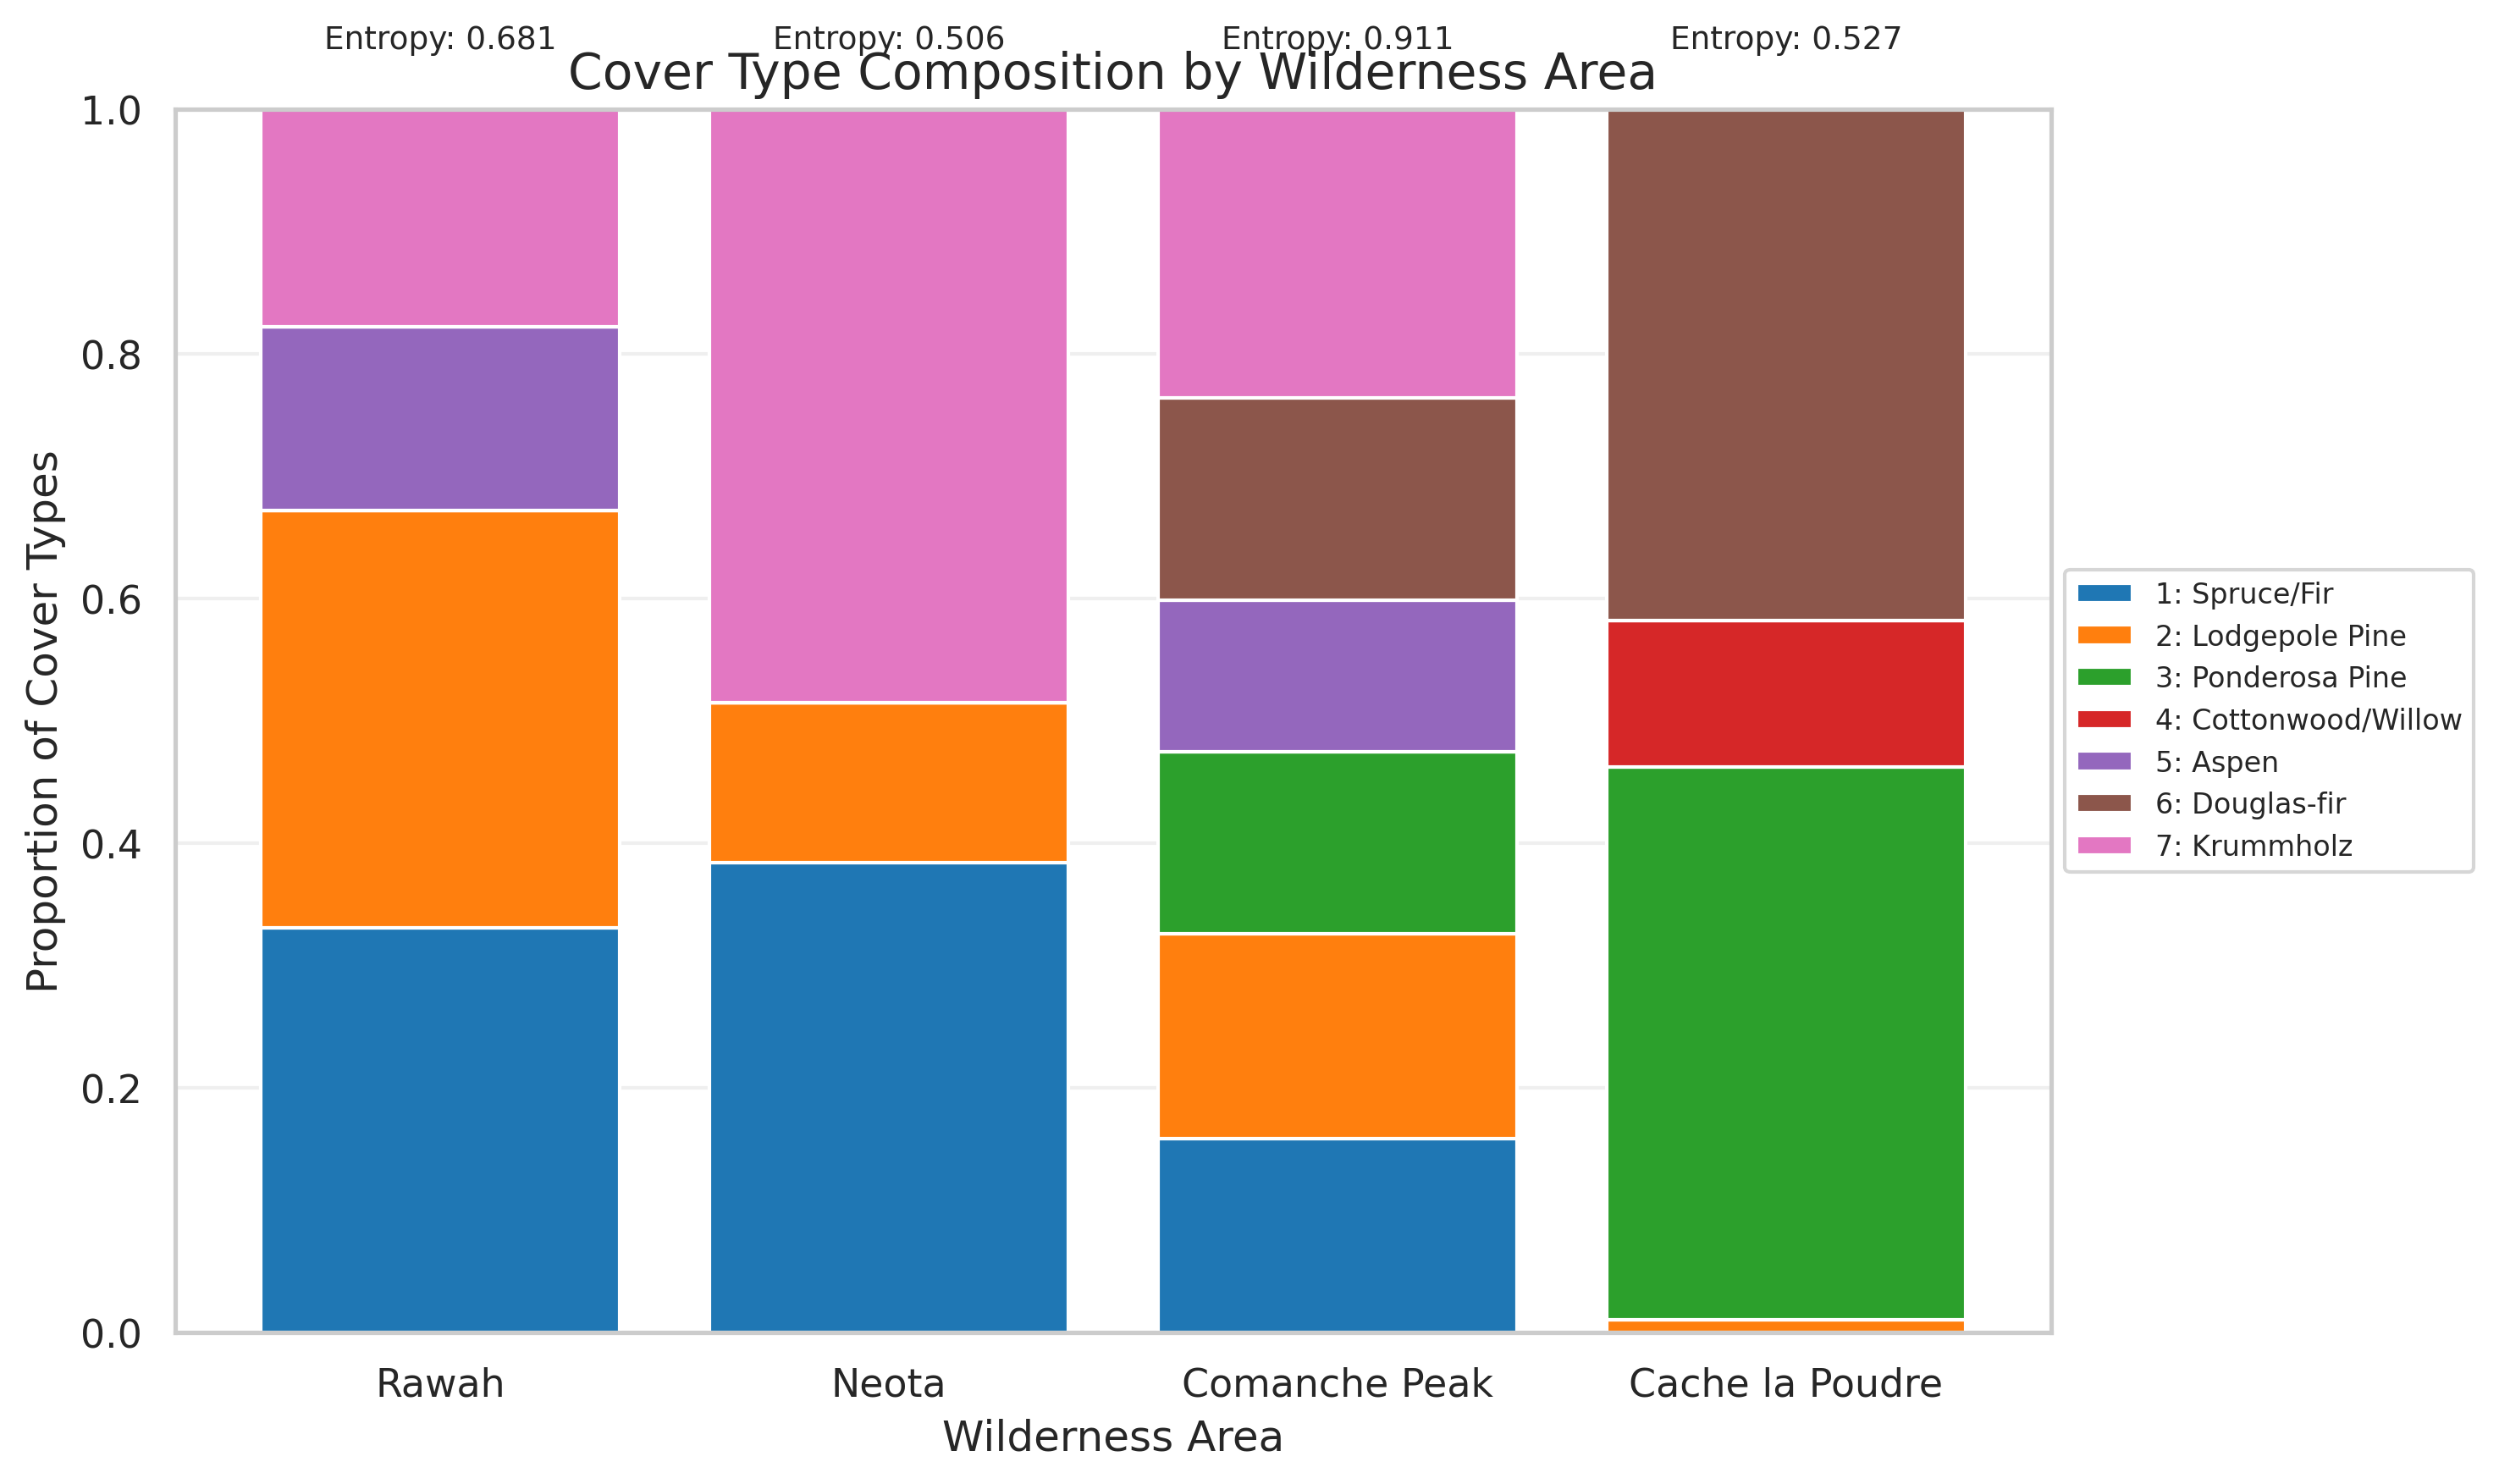
\includegraphics[width=\linewidth]{figures/wilderness_cover_distribution.png}\\[-0.5ex]\small Cover composition\end{minipage}\hfill%
\begin{minipage}{0.48\linewidth}\centering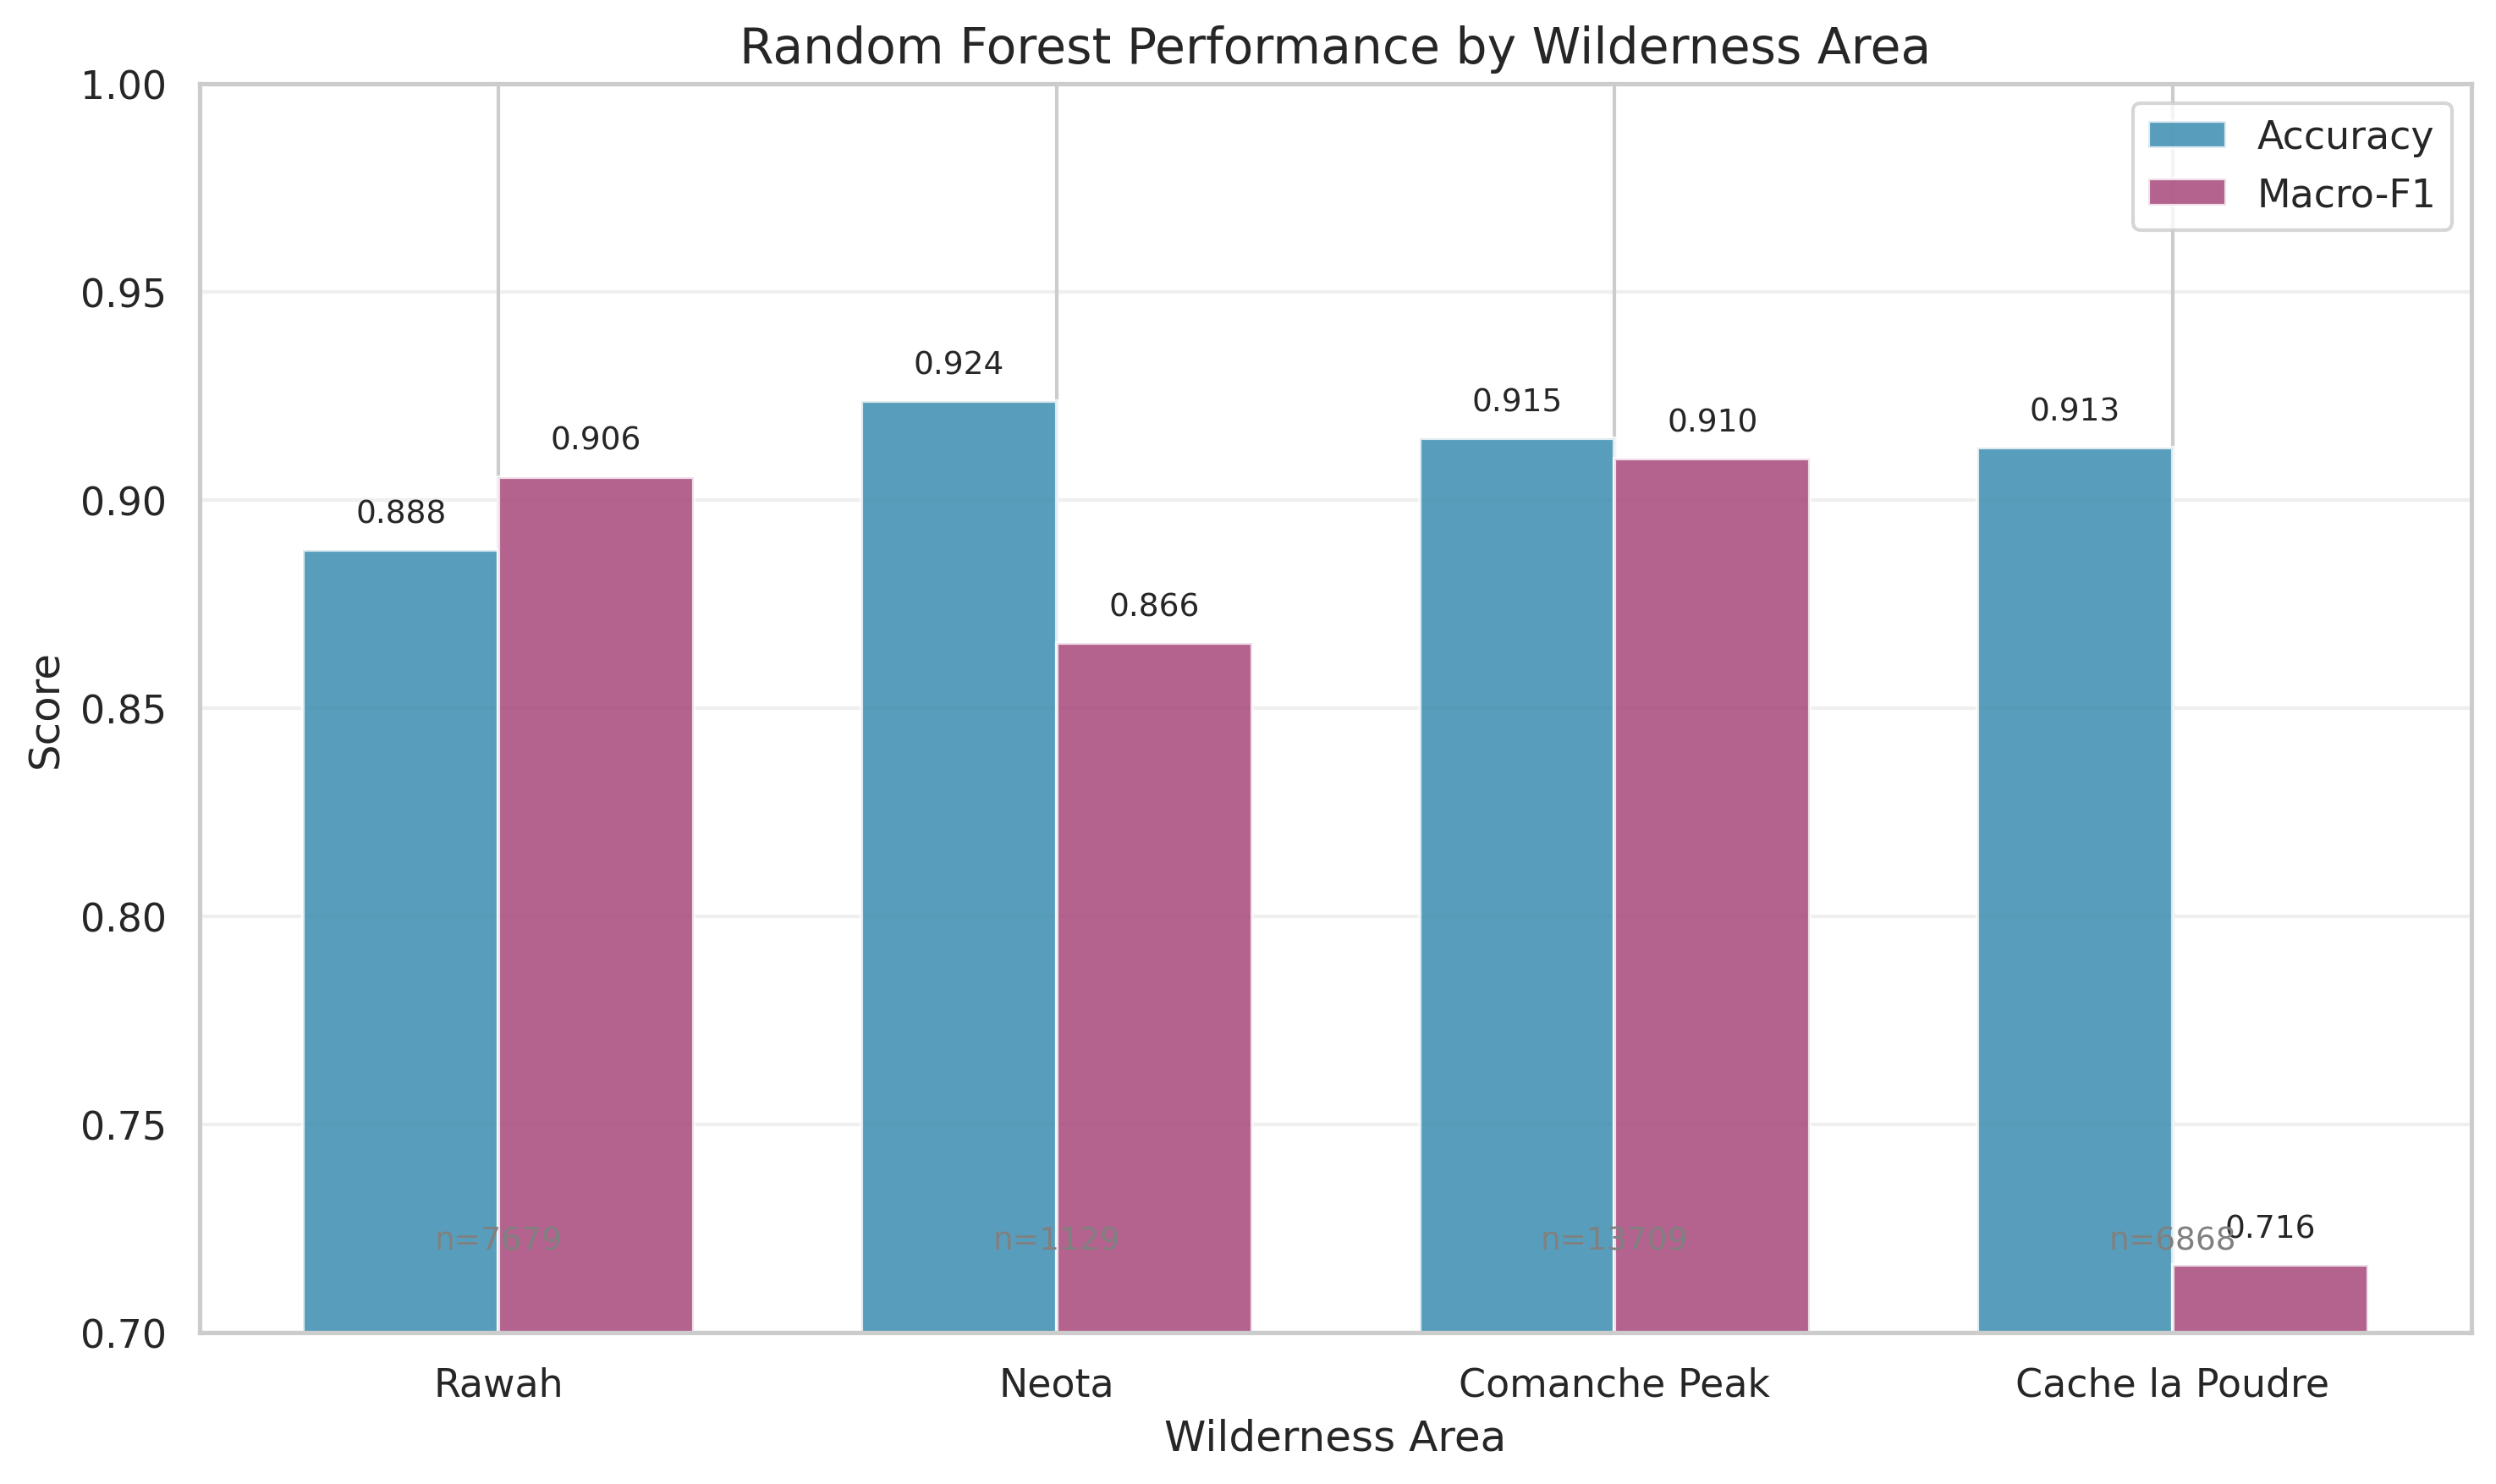
\includegraphics[width=\linewidth]{figures/wilderness_model_metrics.png}\\[-0.5ex]\small Model performance\end{minipage}
\caption{Wilderness-area extension analysis.}
\label{fig:wilderness_extension}
\end{figure}

\section{Prediction: training and testing}
The supervised target is the seven-class \texttt{Cover\_Type}. We use a stratified 120,000-row modeling sample, split 70/30 into 84,000 training and 36,000 test observations. Logistic regression is the linear baseline with class weighting, and a depth-limited decision tree is the simple nonlinear baseline. Both are evaluated on train, test, and full data after training.

\begin{table}[H]
\centering
\caption{Simple-model performance on train, test, and full data.}
\label{tab:simple}
\small
\begin{adjustbox}{max width=\linewidth}
\begin{tabular}{lllll}
\toprule
model & split & accuracy & f1\_macro & AUC\_ovr\_macro \\
\midrule
Logistic Regression & train & 0.594 & 0.473 & 0.923 \\
Logistic Regression & test & 0.593 & 0.471 & 0.923 \\
Logistic Regression & full & 0.593 & 0.472 & 0.923 \\
Decision Tree & train & 0.826 & 0.727 & 0.985 \\
Decision Tree & test & 0.775 & 0.663 & 0.942 \\
Decision Tree & full & 0.782 & 0.671 & 0.949 \\
\bottomrule
\end{tabular}
\end{adjustbox}
\end{table}

\begin{figure}[H]
\centering
\begin{minipage}{0.48\linewidth}\centering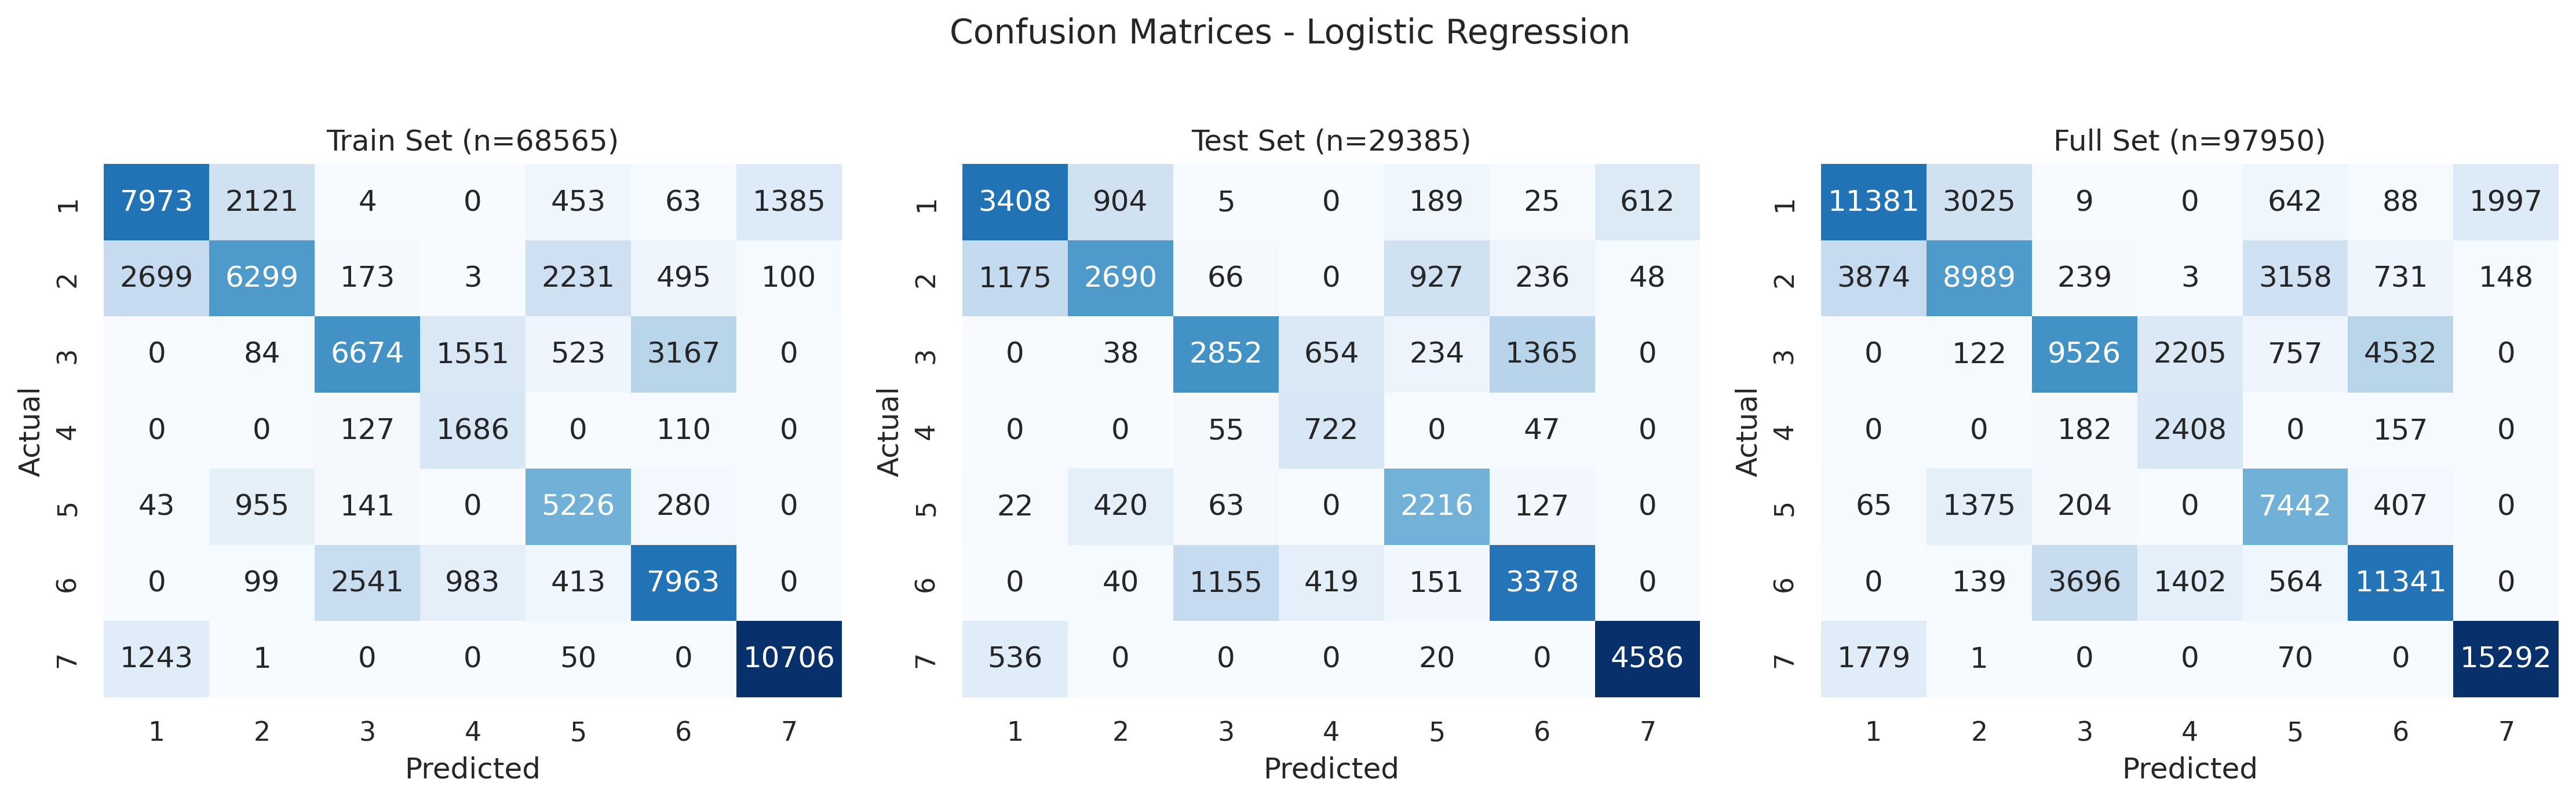
\includegraphics[width=\linewidth]{figures/confusion_logistic_regression.png}\\[-0.5ex]\small Logistic regression\end{minipage}\hfill%
\begin{minipage}{0.48\linewidth}\centering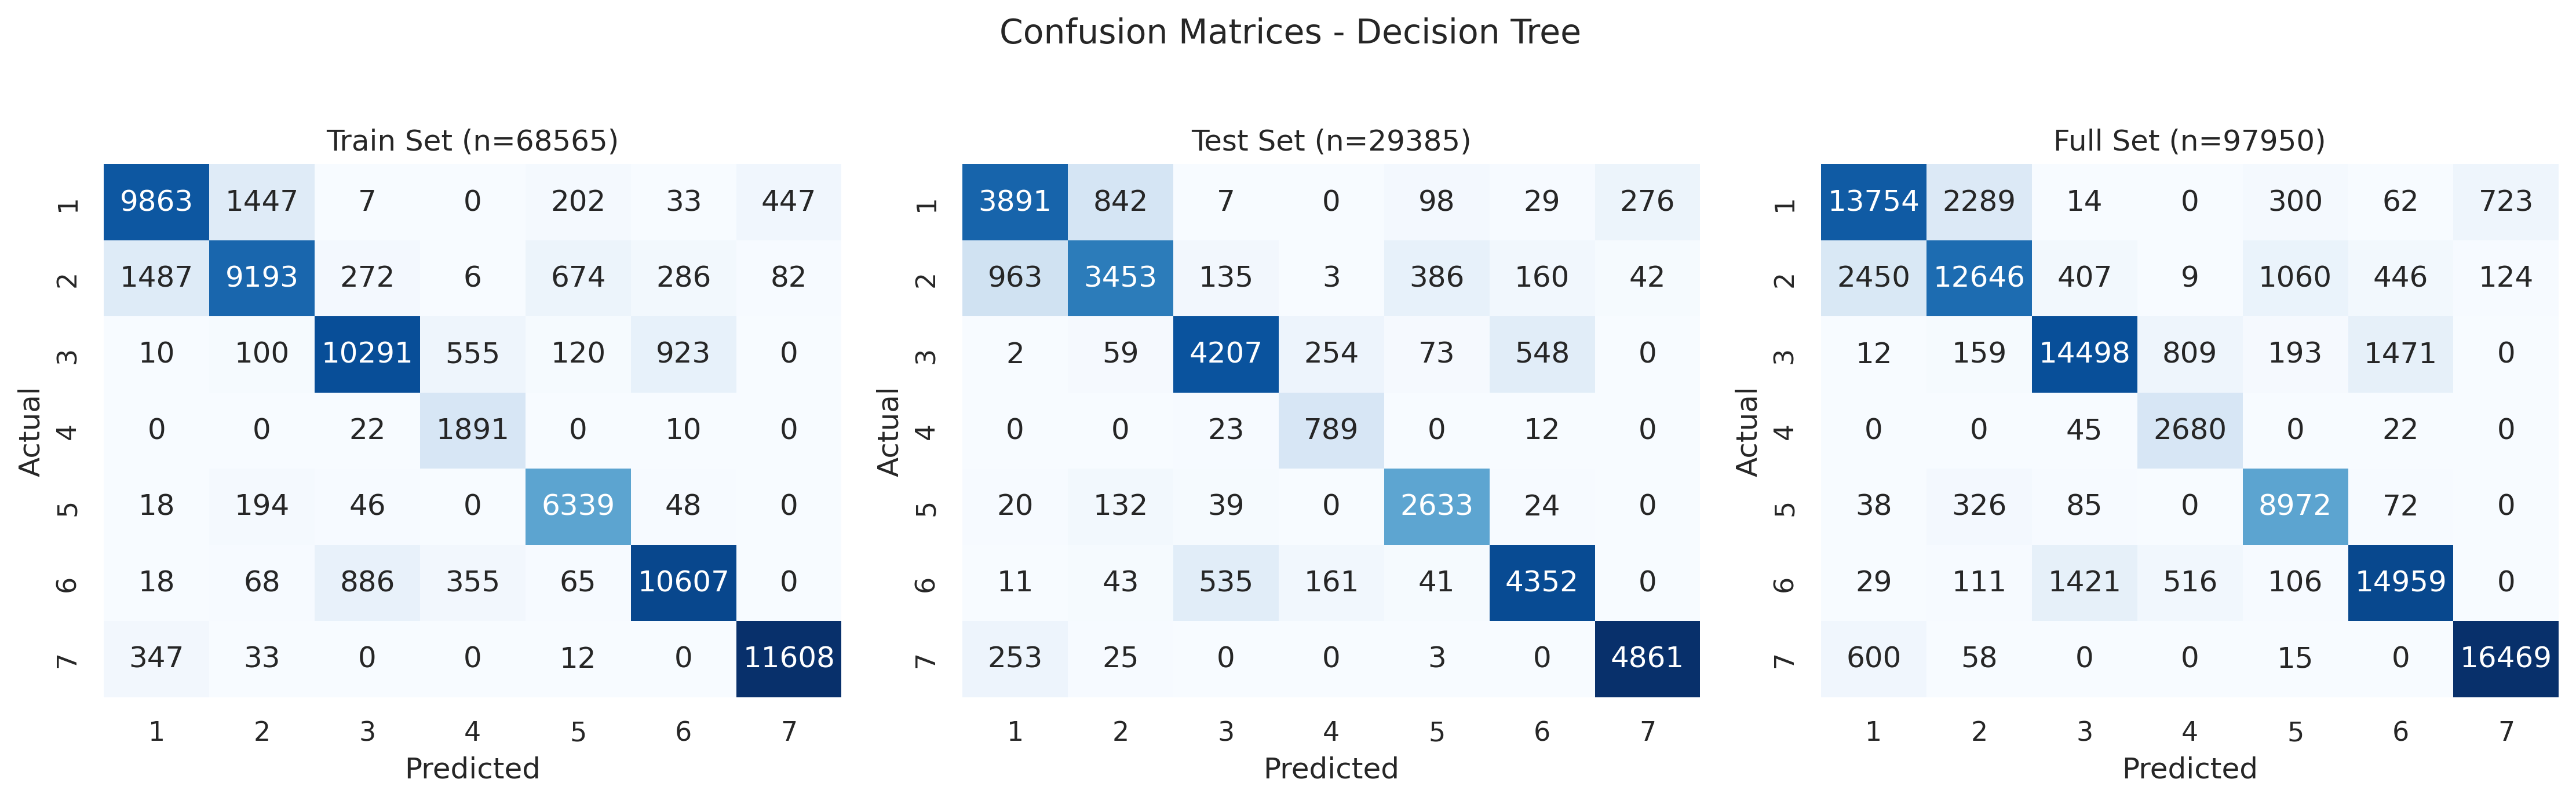
\includegraphics[width=\linewidth]{figures/confusion_decision_tree.png}\\[-0.5ex]\small Decision tree\end{minipage}
\caption{Confusion matrices for the two required simple models.}
\label{fig:confusions}
\end{figure}

\section{Evaluation and model choice}
Logistic regression reaches high macro AUC but weak macro-F1 because the linear boundary struggles with minority classes. The decision tree improves nonlinear separation but still overfits relative to the test set. Random Forest and HistGradientBoosting are added for open-ended model comparison. Random Forest is the best test model with accuracy=0.902, macro-F1=0.845, and macro AUC=0.991. Cross-validation on a separate stratified 36,000-row sample confirms the same ranking.

\begin{table}[H]
\centering
\caption{Test performance across model classes.}
\label{tab:models}
\small
\begin{adjustbox}{max width=\linewidth}
\begin{tabular}{llllll}
\toprule
model & accuracy & precision\_macro & recall\_macro & f1\_macro & AUC\_ovr\_macro \\
\midrule
Logistic Regression & 0.593 & 0.447 & 0.690 & 0.471 & 0.923 \\
Decision Tree & 0.775 & 0.596 & 0.816 & 0.663 & 0.942 \\
Random Forest & 0.902 & 0.853 & 0.840 & 0.845 & 0.991 \\
HistGradientBoosting & 0.869 & 0.866 & 0.806 & 0.831 & 0.985 \\
\bottomrule
\end{tabular}
\end{adjustbox}
\end{table}

\begin{table}[H]
\centering
\caption{Three-fold cross-validation on a stratified sample.}
\label{tab:cv}
\small
\begin{adjustbox}{max width=\linewidth}
\begin{tabular}{llll}
\toprule
model & accuracy\_mean & f1\_macro\_mean & AUC\_ovr\_macro\_mean \\
\midrule
Random Forest & 0.844 & 0.755 & 0.978 \\
HistGradientBoosting & 0.826 & 0.739 & 0.973 \\
Decision Tree & 0.693 & 0.569 & 0.907 \\
Logistic Regression & 0.598 & 0.496 & 0.925 \\
\bottomrule
\end{tabular}
\end{adjustbox}
\end{table}

\begin{figure}[H]
\centering
\begin{minipage}{0.48\linewidth}\centering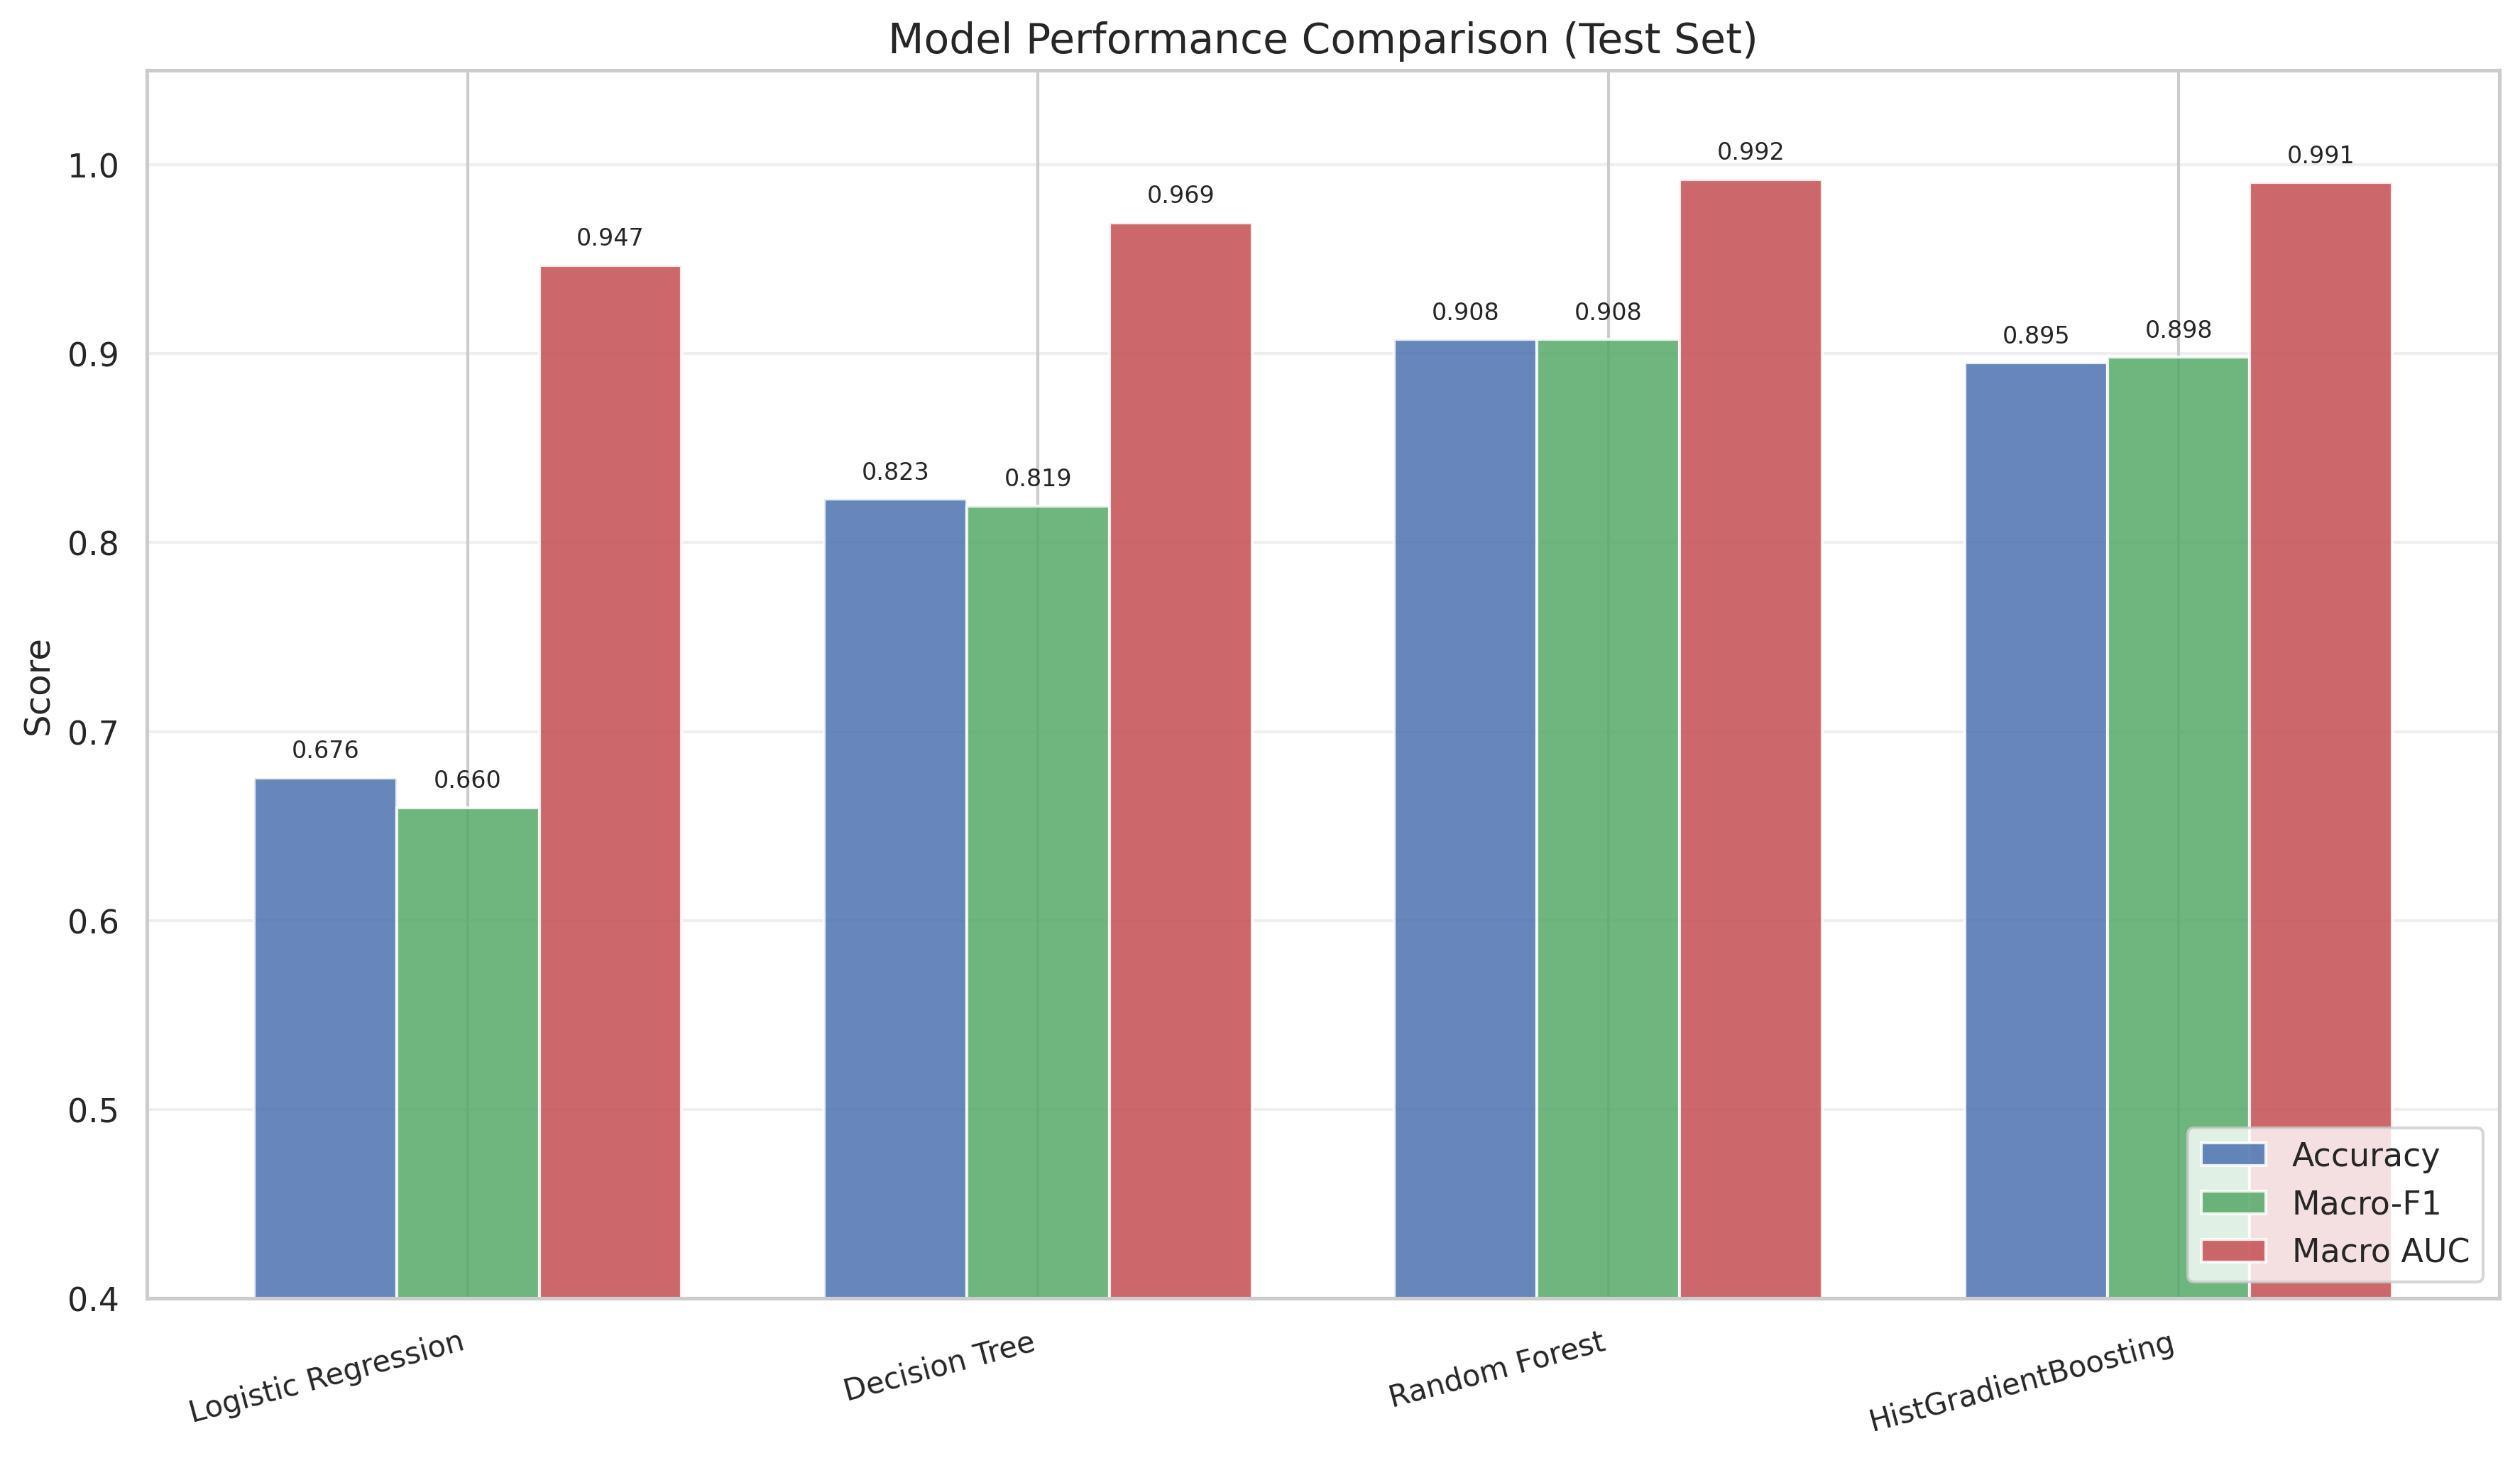
\includegraphics[width=\linewidth]{figures/model_comparison_f1_auc.png}\\[-0.5ex]\small Model metrics\end{minipage}\hfill%
\begin{minipage}{0.48\linewidth}\centering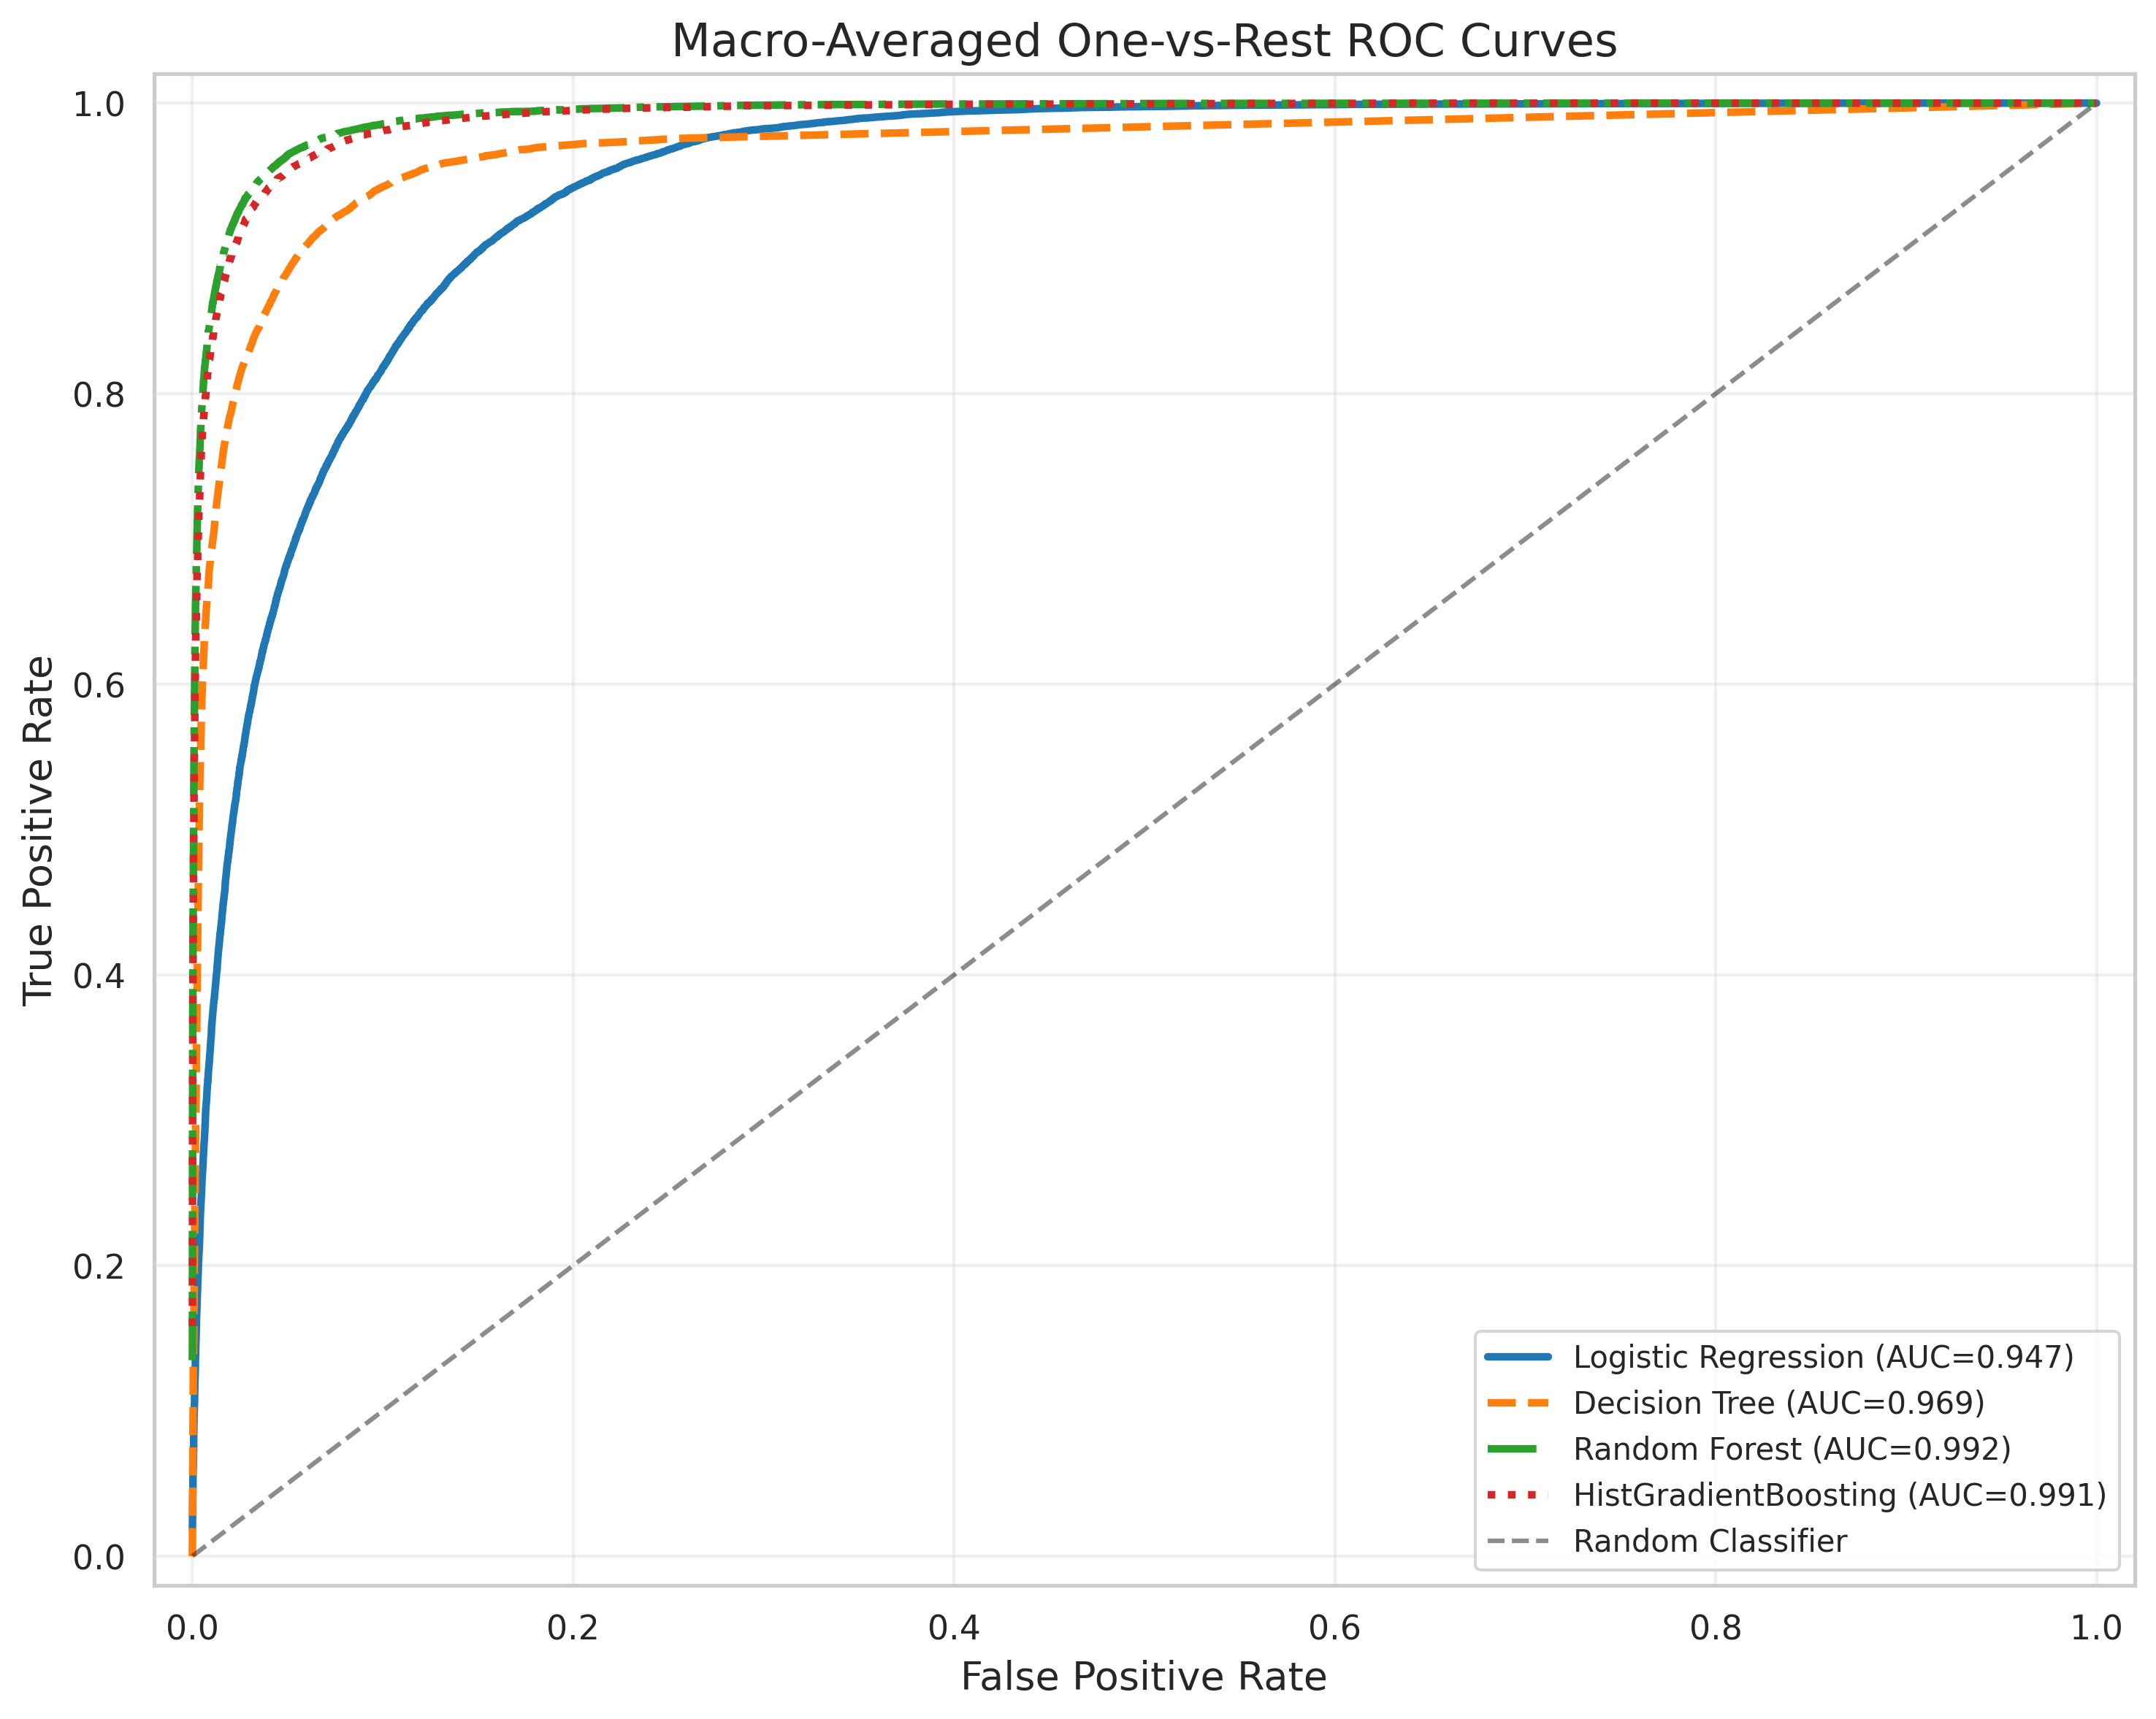
\includegraphics[width=\linewidth]{figures/roc_ovr_models.png}\\[-0.5ex]\small Macro ROC\end{minipage}
\caption{Model comparison and macro one-vs-rest ROC curves.}
\label{fig:model_choice}
\end{figure}

\section{Open-ended exploration}
\subsection{Feature importance and ablation}
Random Forest impurity importance and sampled permutation importance both rank Elevation as the dominant feature, followed by road/fire/hydrology distances and hillshade. Feature-group ablation with HistGradientBoosting shows that topographic variables alone are already strong, but soil indicators add useful predictive signal; wilderness indicators alone are weak.

\begin{table}[H]
\centering
\caption{Top Random Forest impurity importances.}
\label{tab:feature_importance}
\small
\begin{adjustbox}{max width=\linewidth}
\begin{tabular}{ll}
\toprule
feature & importance \\
\midrule
Elevation & 0.235 \\
Horizontal\_Distance\_To\_Roadways & 0.099 \\
Horizontal\_Distance\_To\_Fire\_Points & 0.077 \\
Horizontal\_Distance\_To\_Hydrology & 0.062 \\
Vertical\_Distance\_To\_Hydrology & 0.050 \\
Hillshade\_9am & 0.049 \\
Aspect & 0.044 \\
Hillshade\_3pm & 0.042 \\
\bottomrule
\end{tabular}
\end{adjustbox}
\end{table}

\begin{table}[H]
\centering
\caption{Feature-group ablation using HistGradientBoosting.}
\label{tab:ablation}
\small
\begin{adjustbox}{max width=\linewidth}
\begin{tabular}{lllll}
\toprule
experiment & n\_features & accuracy & f1\_macro & AUC\_ovr\_macro \\
\midrule
All features & 54 & 0.857 & 0.815 & 0.983 \\
Topographic + soil & 50 & 0.850 & 0.807 & 0.981 \\
Topographic + wilderness & 14 & 0.837 & 0.784 & 0.973 \\
Topographic only & 10 & 0.820 & 0.764 & 0.973 \\
Soil only & 40 & 0.618 & 0.279 & 0.873 \\
Wilderness only & 4 & 0.535 & 0.203 & 0.741 \\
\bottomrule
\end{tabular}
\end{adjustbox}
\end{table}

\begin{figure}[H]
\centering
\begin{minipage}{0.48\linewidth}\centering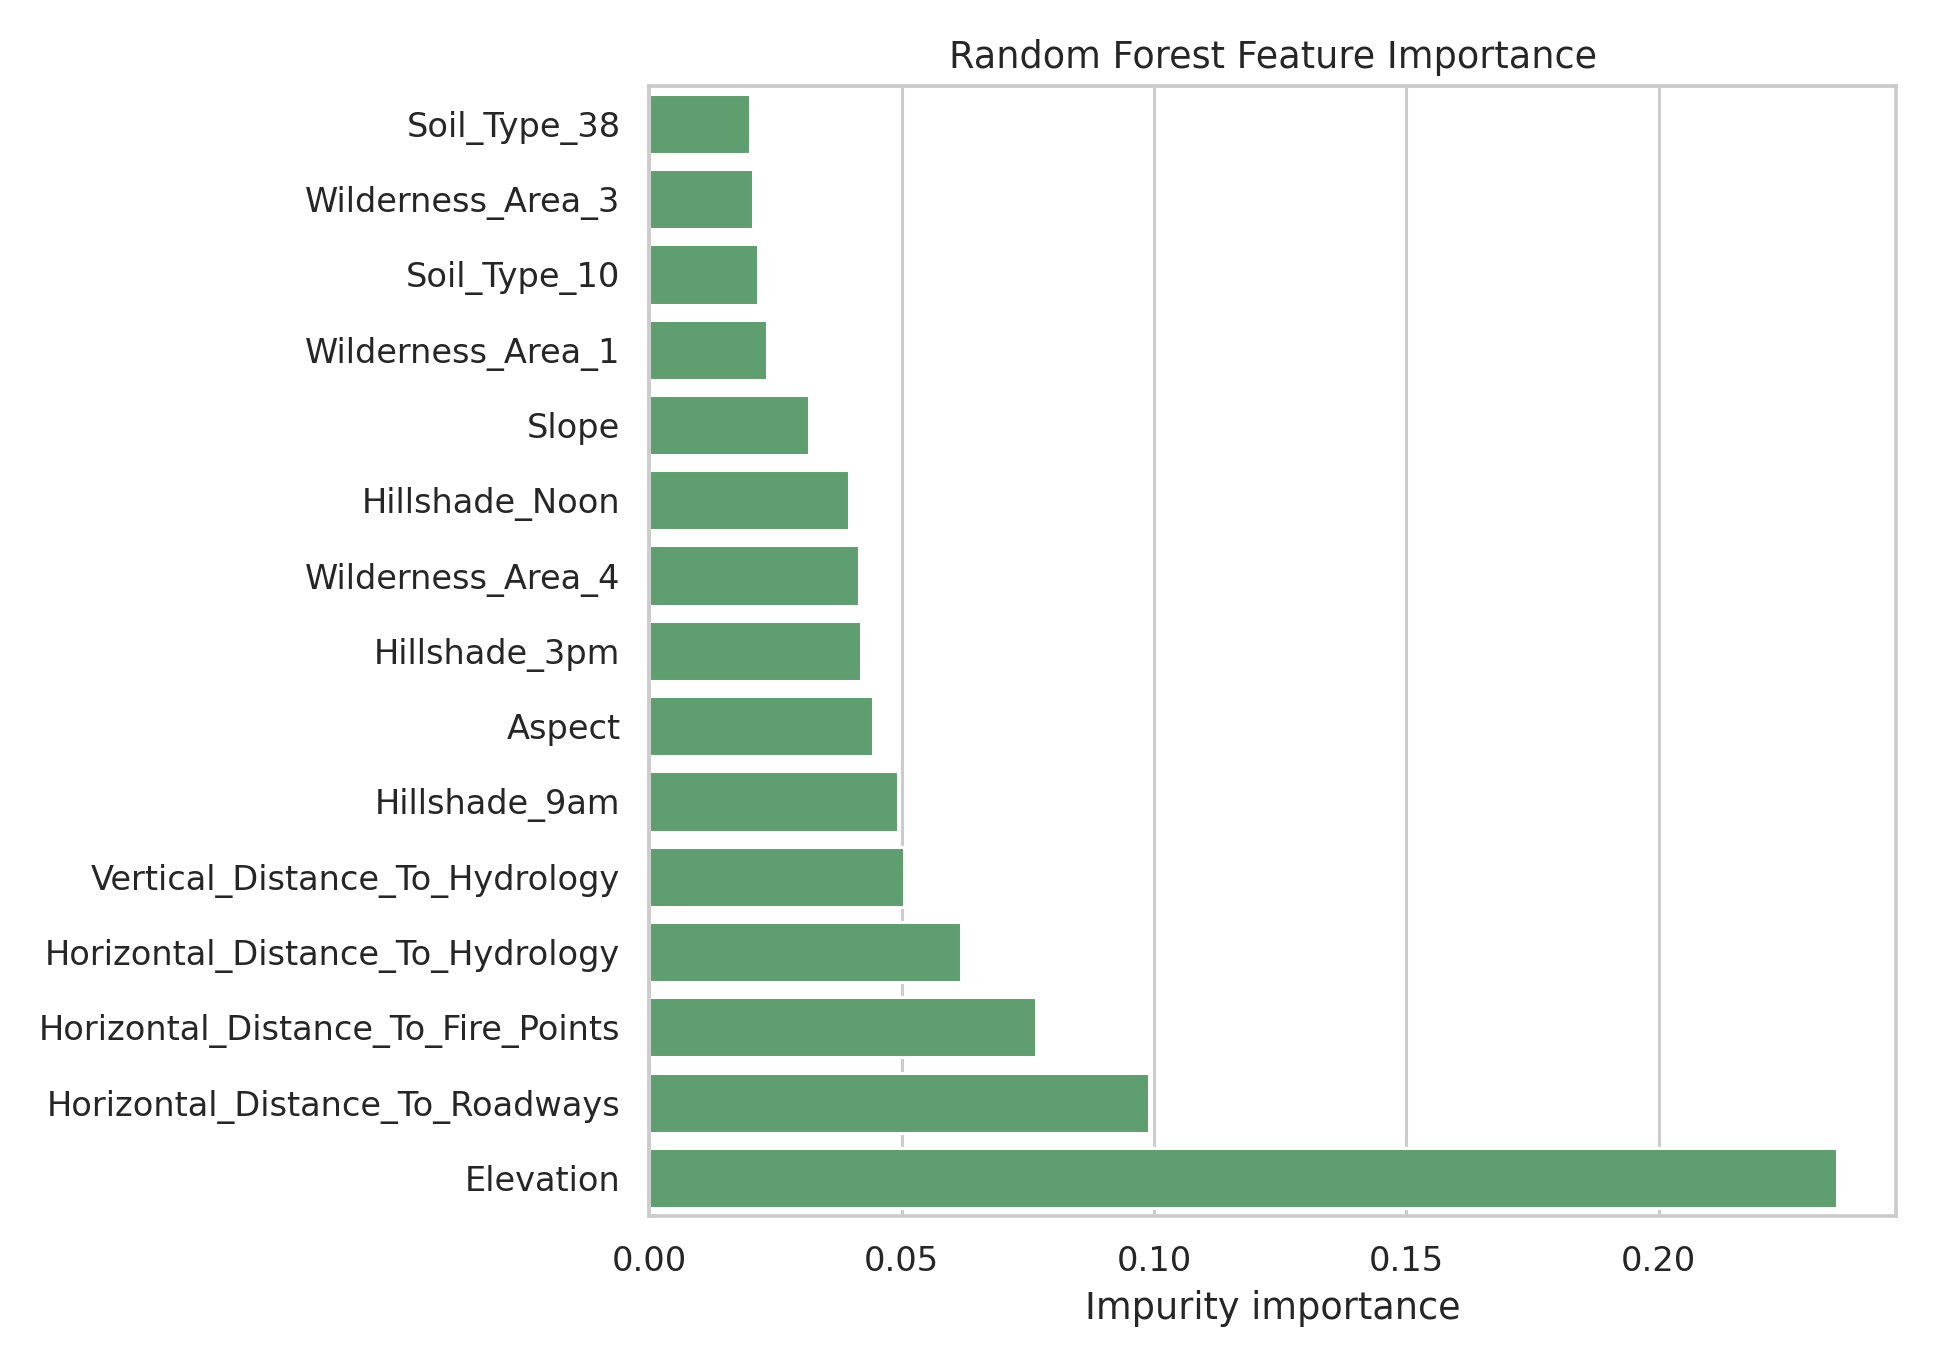
\includegraphics[width=\linewidth]{figures/feature_importance_top15.png}\\[-0.5ex]\small Feature importance\end{minipage}\hfill%
\begin{minipage}{0.48\linewidth}\centering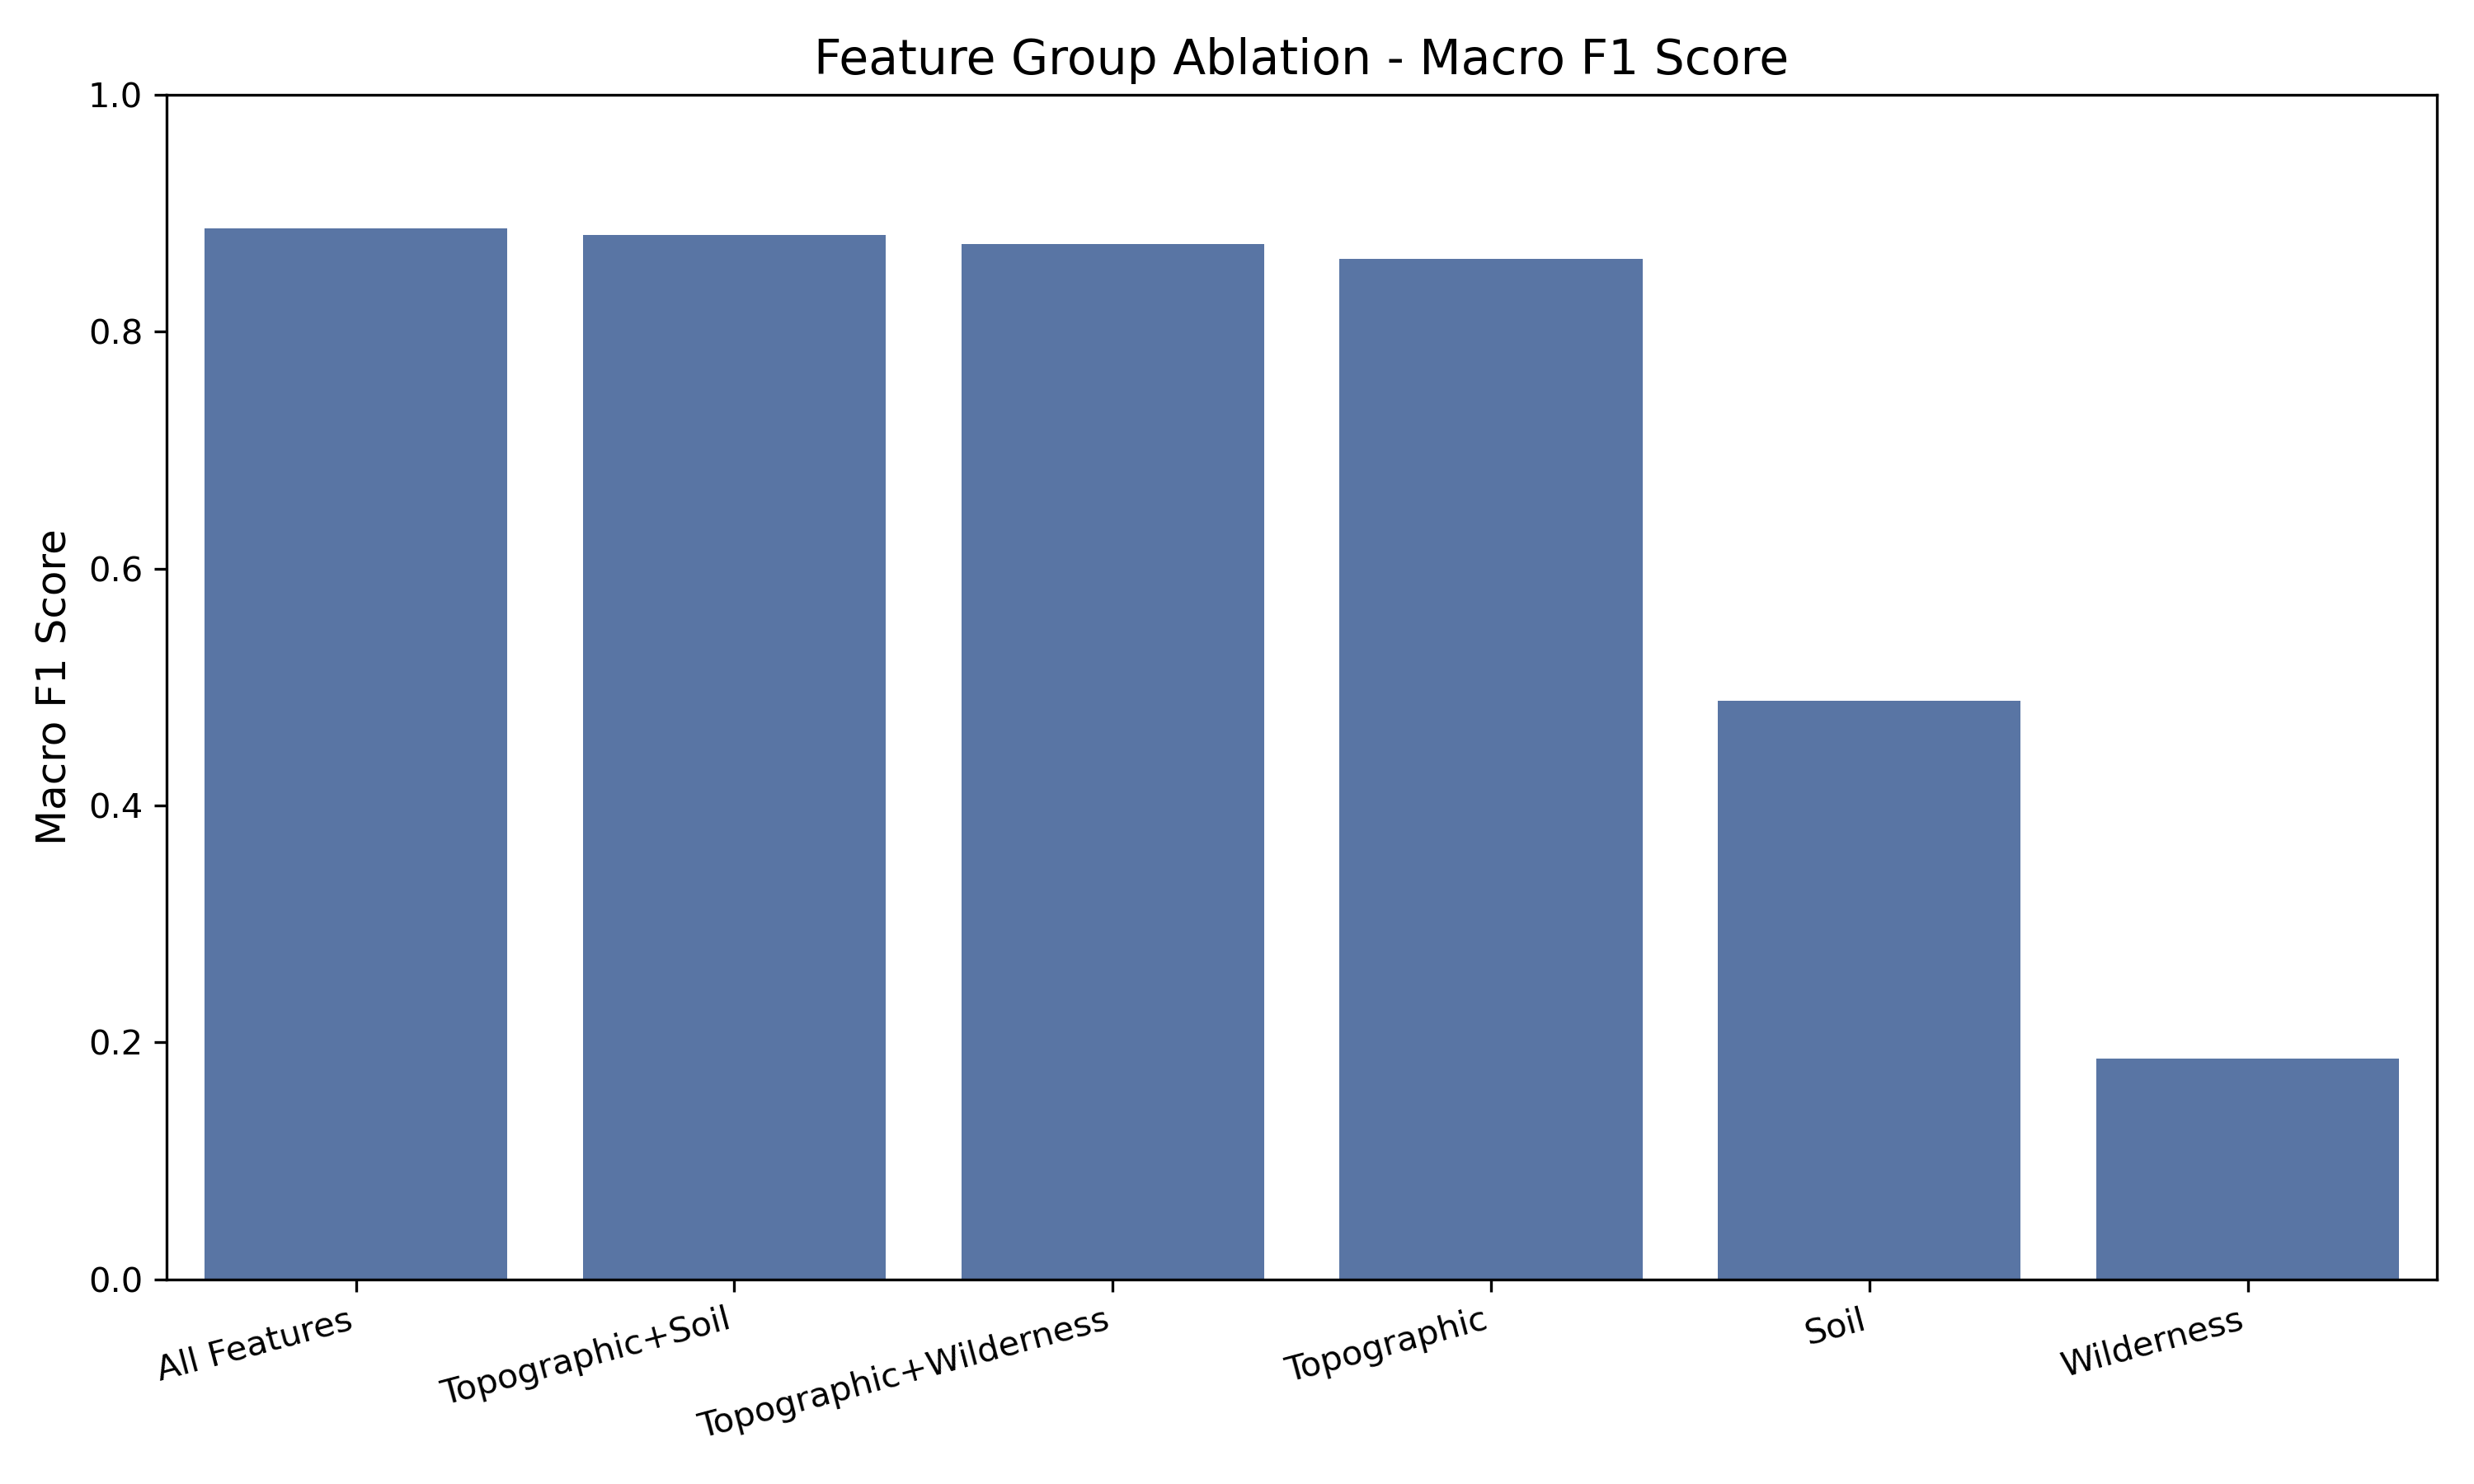
\includegraphics[width=\linewidth]{figures/feature_group_ablation.png}\\[-0.5ex]\small Feature ablation\end{minipage}
\caption{Feature-importance and feature-group analyses.}
\label{fig:features}
\end{figure}

\subsection{Calibration, robustness, and errors}
HistGradientBoosting has the lowest top-label expected calibration error, while Random Forest has the best accuracy and macro-F1 but is under-confident on average. Accuracy also rises in the highest elevation band, indicating that high-elevation classes are easier to separate. Class-level recall shows Aspen and Douglas-fir are harder than the dominant classes.

\begin{table}[H]
\centering
\caption{Top-label calibration summary.}
\label{tab:calibration}
\small
\begin{adjustbox}{max width=\linewidth}
\begin{tabular}{lllll}
\toprule
model & multiclass\_brier & expected\_calibration\_error & mean\_confidence & observed\_accuracy \\
\midrule
HistGradientBoosting & 0.194 & 0.047 & 0.822 & 0.869 \\
Logistic Regression & 0.546 & 0.066 & 0.655 & 0.593 \\
Decision Tree & 0.324 & 0.104 & 0.880 & 0.775 \\
Random Forest & 0.178 & 0.128 & 0.775 & 0.902 \\
\bottomrule
\end{tabular}
\end{adjustbox}
\end{table}

\begin{table}[H]
\centering
\caption{Class-level precision, recall, and F1 for the best model.}
\label{tab:class_report}
\small
\begin{adjustbox}{max width=\linewidth}
\begin{tabular}{llllll}
\toprule
Cover\_Type & Cover\_Type\_Name & support & precision & recall & f1 \\
\midrule
1 & Spruce/Fir & 13126 & 0.919 & 0.885 & 0.901 \\
2 & Lodgepole Pine & 17554 & 0.907 & 0.930 & 0.918 \\
3 & Ponderosa Pine & 2215 & 0.852 & 0.924 & 0.887 \\
4 & Cottonwood/Willow & 170 & 0.782 & 0.824 & 0.802 \\
5 & Aspen & 588 & 0.792 & 0.639 & 0.707 \\
6 & Douglas-fir & 1076 & 0.796 & 0.778 & 0.787 \\
7 & Krummholz & 1271 & 0.920 & 0.901 & 0.911 \\
\bottomrule
\end{tabular}
\end{adjustbox}
\end{table}

\begin{figure}[H]
\centering
\begin{minipage}{0.48\linewidth}\centering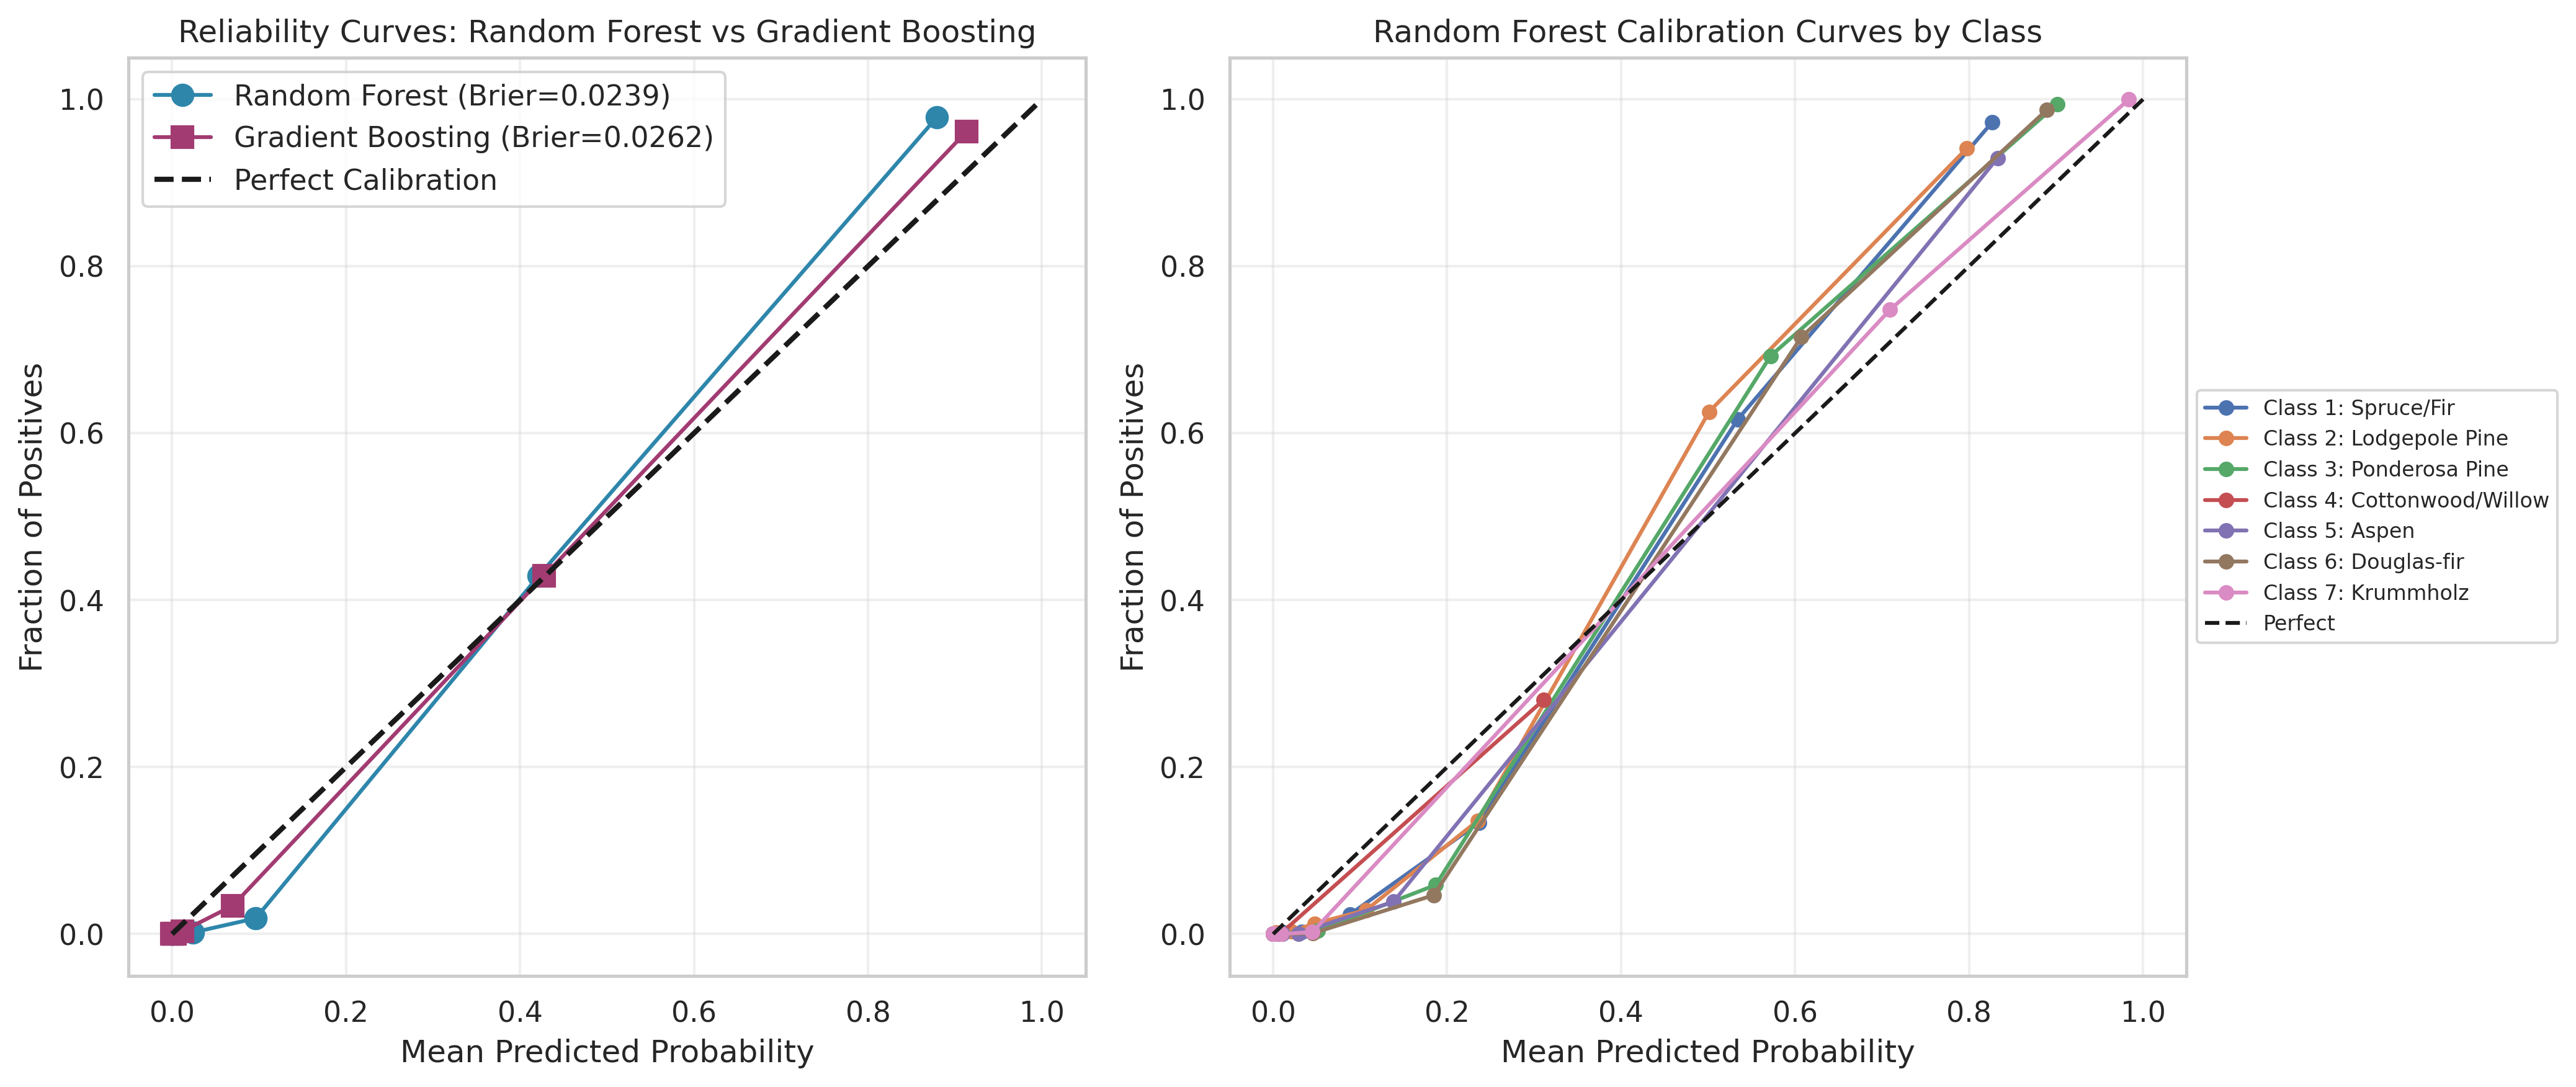
\includegraphics[width=\linewidth]{figures/calibration_reliability.png}\\[-0.5ex]\small Calibration\end{minipage}\hfill%
\begin{minipage}{0.48\linewidth}\centering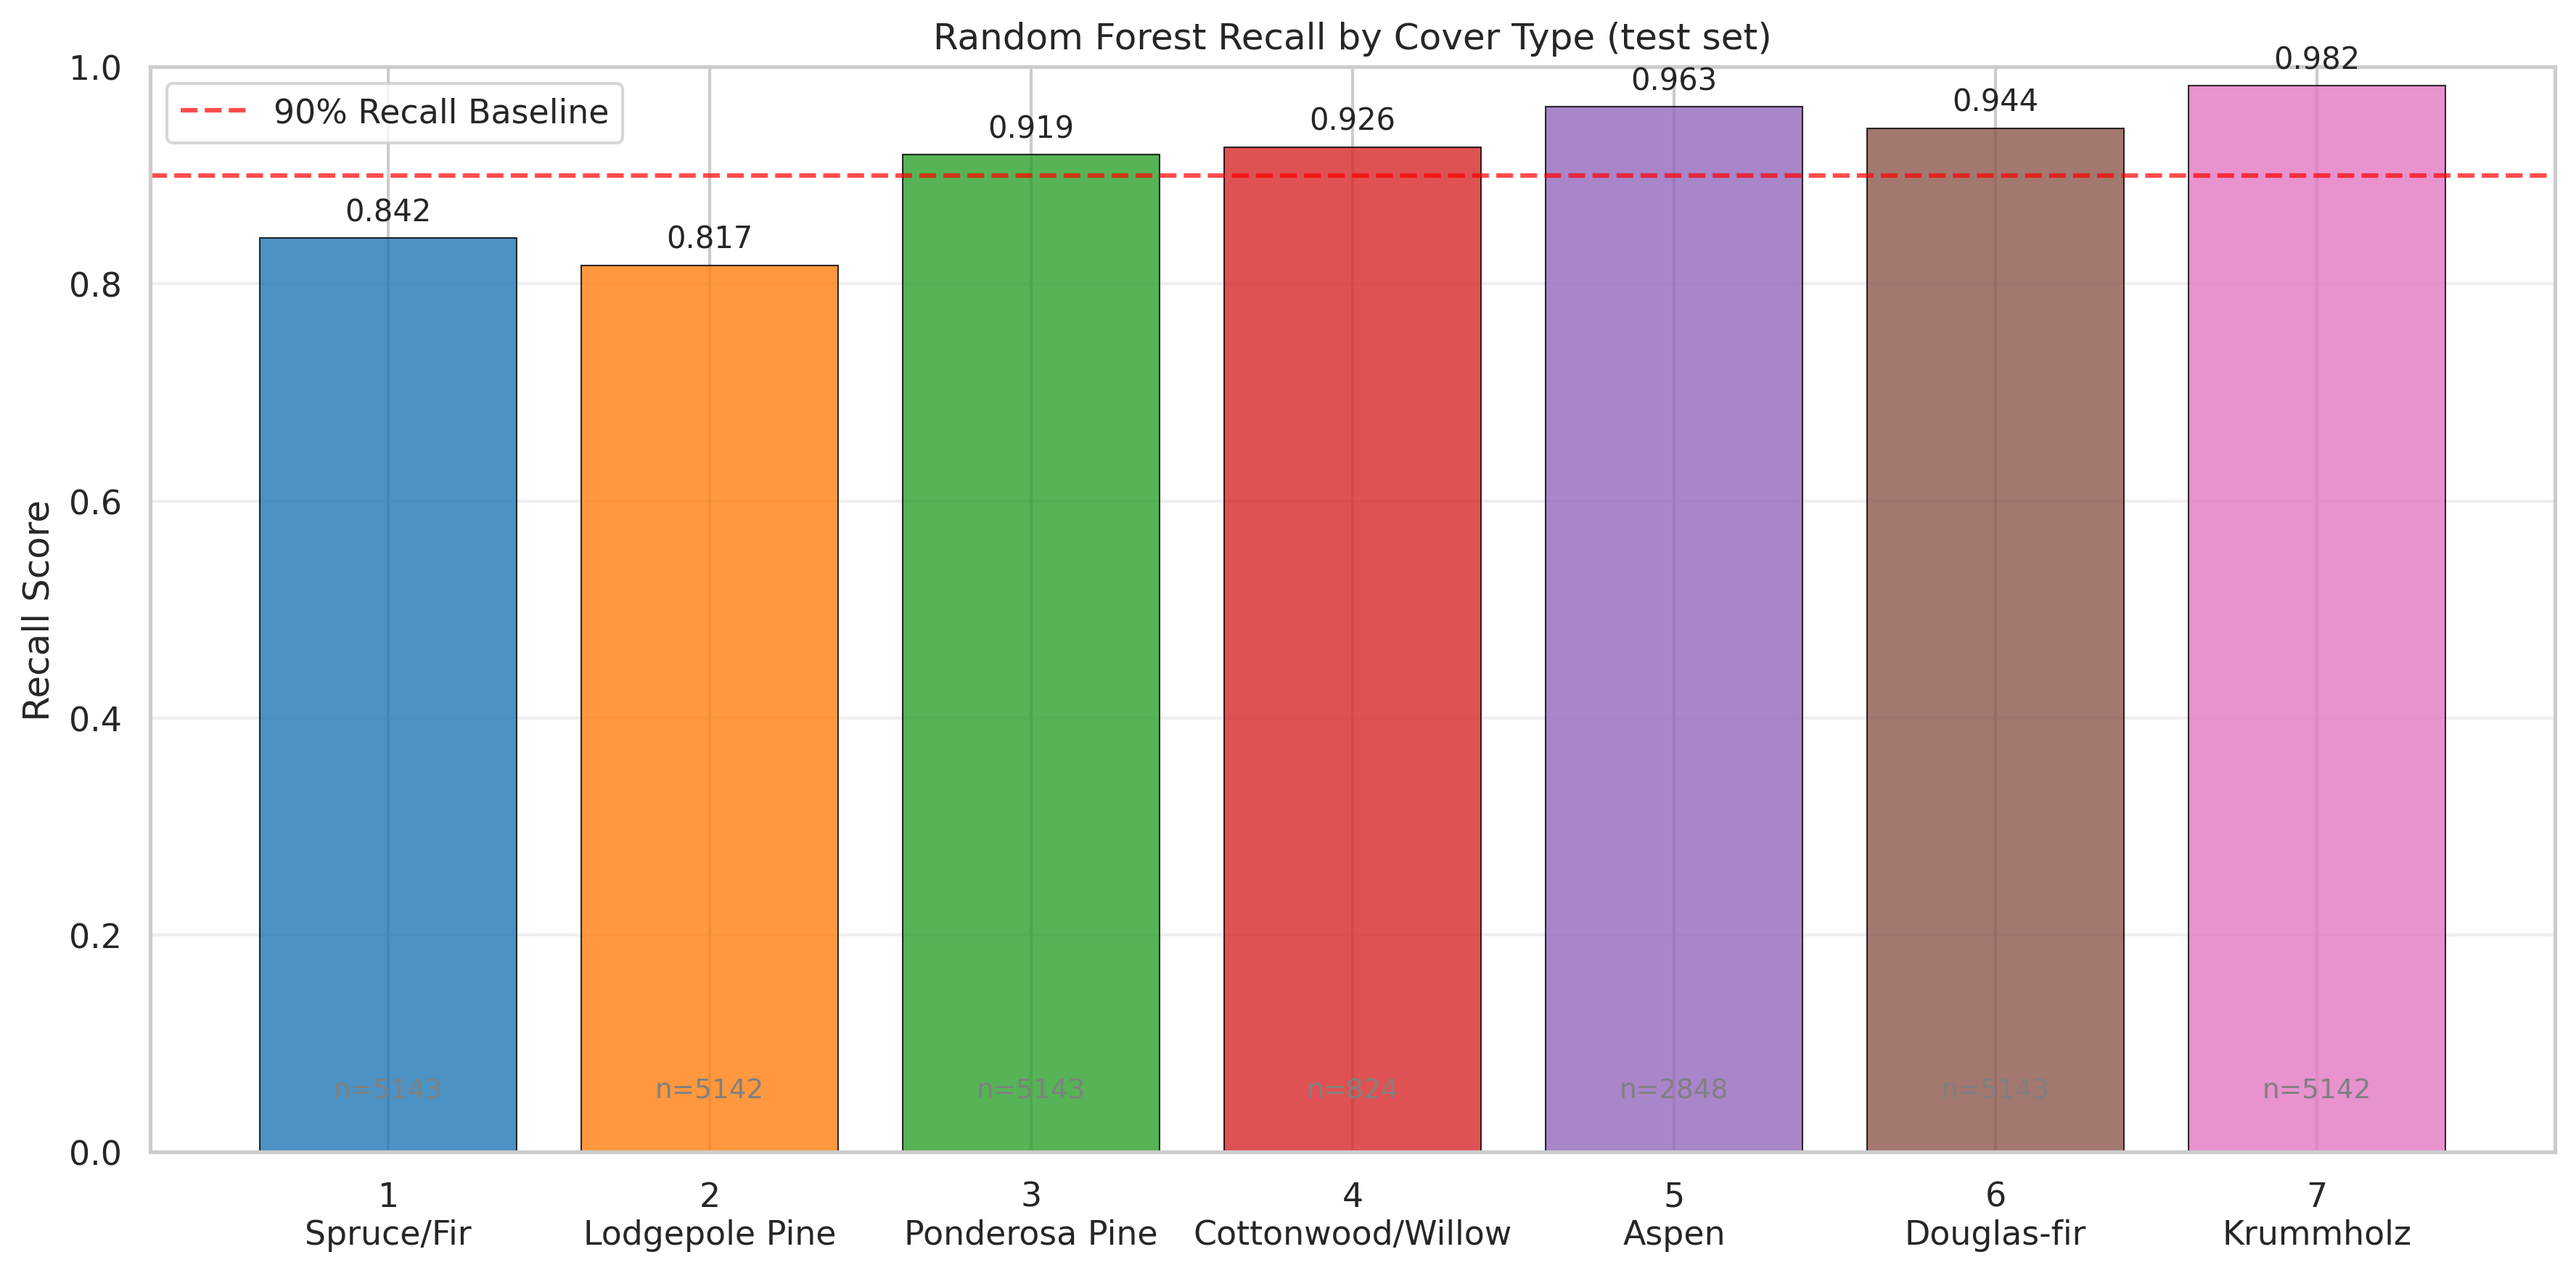
\includegraphics[width=\linewidth]{figures/class_recall_comparison.png}\\[-0.5ex]\small Class recall\end{minipage}
\caption{Calibration and class-level recall diagnostics.}
\label{fig:calibration_class}
\end{figure}

\subsection{Computational optimization}
The optimized workflow implements the cost controls discussed in the project: dtype downcasting, stratified samples for expensive diagnostics, PCA before distance-based analysis, MiniBatchKMeans for scalable clustering, parallel tree ensembles, and manifest-based caches for t-SNE, clustering, and modeling outputs. A warm rebuild hits the heavy-stage caches, making report regeneration fast and auditable.

\begin{figure}[H]
\centering
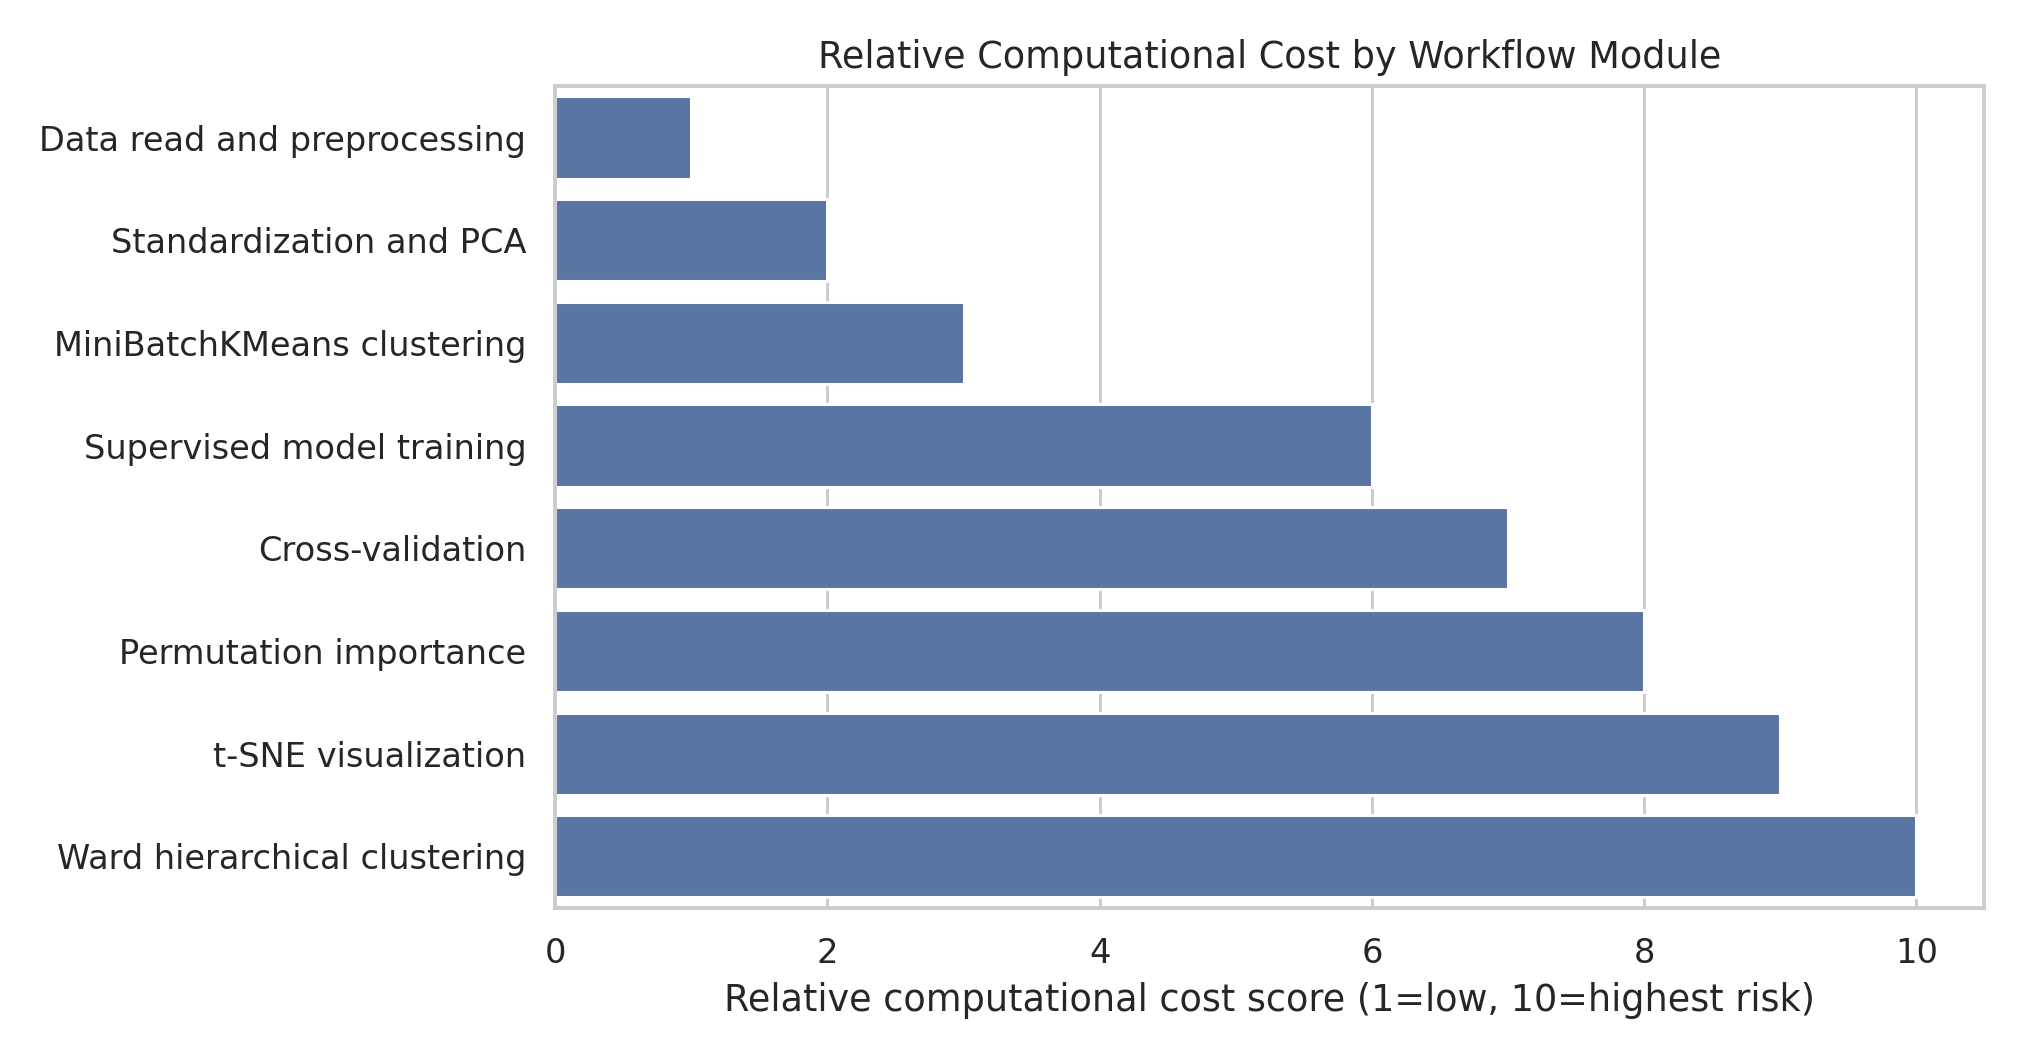
\includegraphics[width=0.82\linewidth]{figures/computational_cost_tiers.png}
\caption{Relative computational cost by workflow module.}
\label{fig:cost}
\end{figure}

\begin{table}[H]
\centering
\caption{Runtime profile after cache-enabled optimization.}
\label{tab:runtime}
\small
\begin{adjustbox}{max width=\linewidth}
\begin{tabular}{lll}
\toprule
stage & seconds & cache\_status \\
\midrule
data\_read\_downcast & 0.88 & computed \\
descriptive\_outputs & 1.00 & computed \\
computational\_cost\_outputs & 0.21 & computed \\
t-SNE & 0.00 & cache\_hit \\
clustering & 6.89 & computed \\
modeling & 135.25 & computed \\
\bottomrule
\end{tabular}
\end{adjustbox}
\end{table}

\section{Conclusion}
The Covertype dataset has strong class imbalance and overlapping ecological classes. Unsupervised clustering exposes broad terrain and regional structure, but the near-zero ARI against \texttt{Cover\_Type} only shows that these natural partitions are not the same object as the seven supervised labels. The Wilderness Area extension makes this distinction explicit by comparing cover-type composition and held-out model performance across regions. Supervised tree ensembles are substantially more effective, with Random Forest giving the best overall classification performance and HistGradientBoosting offering better calibration. Elevation is the strongest feature, but road/fire/hydrology distances, soil context, and regional evaluation all add meaningful interpretation. For deployment-style interpretation, the model should be reported with macro metrics, class-level recall, calibration, terrain-band and wilderness-area performance, and explicit sampling assumptions.

\section*{References}
\begin{enumerate}[leftmargin=*, itemsep=0.25em]
  \item UCI Machine Learning Repository. Covertype dataset. \url{https://archive.ics.uci.edu/ml/datasets/covertype}.
  \item Blackard, Jock A. and Dean, Denis J. Comparative Accuracies of Artificial Neural Networks and Discriminant Analysis in Predicting Forest Cover Types from Cartographic Variables. \emph{Computers and Electronics in Agriculture}, 1999.
  \item Pedregosa et al. Scikit-learn: Machine Learning in Python. \emph{Journal of Machine Learning Research}, 2011.
  \item van der Maaten and Hinton. Visualizing Data using t-SNE. \emph{Journal of Machine Learning Research}, 2008.
\end{enumerate}

\section*{Credit and GenAI use}
Analysis code, figures, and report text were generated reproducibly in this repository. Group-member contribution details should be finalized by the project team before submission. OpenAI Codex was used to draft, refactor, and validate the analysis workflow and report.

\end{document}
